% Options for packages loaded elsewhere
\PassOptionsToPackage{unicode}{hyperref}
\PassOptionsToPackage{hyphens}{url}
%
\documentclass[
  8pt,
  ignorenonframetext,
]{beamer}
\usepackage{pgfpages}
\setbeamertemplate{caption}[numbered]
\setbeamertemplate{caption label separator}{: }
\setbeamercolor{caption name}{fg=normal text.fg}
\beamertemplatenavigationsymbolsempty
% Prevent slide breaks in the middle of a paragraph
\widowpenalties 1 10000
\raggedbottom
\setbeamertemplate{part page}{
  \centering
  \begin{beamercolorbox}[sep=16pt,center]{part title}
    \usebeamerfont{part title}\insertpart\par
  \end{beamercolorbox}
}
\setbeamertemplate{section page}{
  \centering
  \begin{beamercolorbox}[sep=12pt,center]{part title}
    \usebeamerfont{section title}\insertsection\par
  \end{beamercolorbox}
}
\setbeamertemplate{subsection page}{
  \centering
  \begin{beamercolorbox}[sep=8pt,center]{part title}
    \usebeamerfont{subsection title}\insertsubsection\par
  \end{beamercolorbox}
}
\AtBeginPart{
  \frame{\partpage}
}
\AtBeginSection{
  \ifbibliography
  \else
    \frame{\sectionpage}
  \fi
}
\AtBeginSubsection{
  \frame{\subsectionpage}
}
\usepackage{amsmath,amssymb}
\usepackage{lmodern}
\usepackage{ifxetex,ifluatex}
\ifnum 0\ifxetex 1\fi\ifluatex 1\fi=0 % if pdftex
  \usepackage[T1]{fontenc}
  \usepackage[utf8]{inputenc}
  \usepackage{textcomp} % provide euro and other symbols
\else % if luatex or xetex
  \usepackage{unicode-math}
  \defaultfontfeatures{Scale=MatchLowercase}
  \defaultfontfeatures[\rmfamily]{Ligatures=TeX,Scale=1}
\fi
% Use upquote if available, for straight quotes in verbatim environments
\IfFileExists{upquote.sty}{\usepackage{upquote}}{}
\IfFileExists{microtype.sty}{% use microtype if available
  \usepackage[]{microtype}
  \UseMicrotypeSet[protrusion]{basicmath} % disable protrusion for tt fonts
}{}
\makeatletter
\@ifundefined{KOMAClassName}{% if non-KOMA class
  \IfFileExists{parskip.sty}{%
    \usepackage{parskip}
  }{% else
    \setlength{\parindent}{0pt}
    \setlength{\parskip}{6pt plus 2pt minus 1pt}}
}{% if KOMA class
  \KOMAoptions{parskip=half}}
\makeatother
\usepackage{xcolor}
\IfFileExists{xurl.sty}{\usepackage{xurl}}{} % add URL line breaks if available
\IfFileExists{bookmark.sty}{\usepackage{bookmark}}{\usepackage{hyperref}}
\hypersetup{
  hidelinks,
  pdfcreator={LaTeX via pandoc}}
\urlstyle{same} % disable monospaced font for URLs
\newif\ifbibliography
\usepackage{color}
\usepackage{fancyvrb}
\newcommand{\VerbBar}{|}
\newcommand{\VERB}{\Verb[commandchars=\\\{\}]}
\DefineVerbatimEnvironment{Highlighting}{Verbatim}{commandchars=\\\{\}}
% Add ',fontsize=\small' for more characters per line
\usepackage{framed}
\definecolor{shadecolor}{RGB}{248,248,248}
\newenvironment{Shaded}{\begin{snugshade}}{\end{snugshade}}
\newcommand{\AlertTok}[1]{\textcolor[rgb]{0.94,0.16,0.16}{#1}}
\newcommand{\AnnotationTok}[1]{\textcolor[rgb]{0.56,0.35,0.01}{\textbf{\textit{#1}}}}
\newcommand{\AttributeTok}[1]{\textcolor[rgb]{0.77,0.63,0.00}{#1}}
\newcommand{\BaseNTok}[1]{\textcolor[rgb]{0.00,0.00,0.81}{#1}}
\newcommand{\BuiltInTok}[1]{#1}
\newcommand{\CharTok}[1]{\textcolor[rgb]{0.31,0.60,0.02}{#1}}
\newcommand{\CommentTok}[1]{\textcolor[rgb]{0.56,0.35,0.01}{\textit{#1}}}
\newcommand{\CommentVarTok}[1]{\textcolor[rgb]{0.56,0.35,0.01}{\textbf{\textit{#1}}}}
\newcommand{\ConstantTok}[1]{\textcolor[rgb]{0.00,0.00,0.00}{#1}}
\newcommand{\ControlFlowTok}[1]{\textcolor[rgb]{0.13,0.29,0.53}{\textbf{#1}}}
\newcommand{\DataTypeTok}[1]{\textcolor[rgb]{0.13,0.29,0.53}{#1}}
\newcommand{\DecValTok}[1]{\textcolor[rgb]{0.00,0.00,0.81}{#1}}
\newcommand{\DocumentationTok}[1]{\textcolor[rgb]{0.56,0.35,0.01}{\textbf{\textit{#1}}}}
\newcommand{\ErrorTok}[1]{\textcolor[rgb]{0.64,0.00,0.00}{\textbf{#1}}}
\newcommand{\ExtensionTok}[1]{#1}
\newcommand{\FloatTok}[1]{\textcolor[rgb]{0.00,0.00,0.81}{#1}}
\newcommand{\FunctionTok}[1]{\textcolor[rgb]{0.00,0.00,0.00}{#1}}
\newcommand{\ImportTok}[1]{#1}
\newcommand{\InformationTok}[1]{\textcolor[rgb]{0.56,0.35,0.01}{\textbf{\textit{#1}}}}
\newcommand{\KeywordTok}[1]{\textcolor[rgb]{0.13,0.29,0.53}{\textbf{#1}}}
\newcommand{\NormalTok}[1]{#1}
\newcommand{\OperatorTok}[1]{\textcolor[rgb]{0.81,0.36,0.00}{\textbf{#1}}}
\newcommand{\OtherTok}[1]{\textcolor[rgb]{0.56,0.35,0.01}{#1}}
\newcommand{\PreprocessorTok}[1]{\textcolor[rgb]{0.56,0.35,0.01}{\textit{#1}}}
\newcommand{\RegionMarkerTok}[1]{#1}
\newcommand{\SpecialCharTok}[1]{\textcolor[rgb]{0.00,0.00,0.00}{#1}}
\newcommand{\SpecialStringTok}[1]{\textcolor[rgb]{0.31,0.60,0.02}{#1}}
\newcommand{\StringTok}[1]{\textcolor[rgb]{0.31,0.60,0.02}{#1}}
\newcommand{\VariableTok}[1]{\textcolor[rgb]{0.00,0.00,0.00}{#1}}
\newcommand{\VerbatimStringTok}[1]{\textcolor[rgb]{0.31,0.60,0.02}{#1}}
\newcommand{\WarningTok}[1]{\textcolor[rgb]{0.56,0.35,0.01}{\textbf{\textit{#1}}}}
\usepackage{longtable,booktabs,array}
\usepackage{calc} % for calculating minipage widths
\usepackage{caption}
% Make caption package work with longtable
\makeatletter
\def\fnum@table{\tablename~\thetable}
\makeatother
\setlength{\emergencystretch}{3em} % prevent overfull lines
\providecommand{\tightlist}{%
  \setlength{\itemsep}{0pt}\setlength{\parskip}{0pt}}
\setcounter{secnumdepth}{-\maxdimen} % remove section numbering
% type setting
% ------------------------------------------------------------------------------
\usepackage[german]{babel}     

% fonts
% ------------------------------------------------------------------------------
\usefonttheme{professionalfonts}

% slide title and horizontal line
% ------------------------------------------------------------------------------
\setbeamertemplate{frametitle}{%
    \vskip-30pt \color{black}\large%
    \begin{minipage}[b][23pt]{120mm}%
    \flushleft\insertframetitle%
    \end{minipage}%
}

\setbeamertemplate{headline}										
{
\vskip10pt\hfill\hspace{3.5mm} 										 
\vskip15pt\color{black}\rule{\textwidth}{0.4pt} 					 
}

% slide number
% ---------------------------------------------------------------
\setbeamertemplate{navigation symbols}{}
\setbeamertemplate{footline}
{
\vskip5pt
\vskip2pt
\makebox[123mm]{\hspace{7.5mm}
\hfill Allgemeines Lineares Modell $\vert$ 
\copyright $ $ 2022 Dirk Ostwald CC BY-NC-SA 4.0 $\vert$ 
Folie \insertframenumber}
\vskip4pt
}

% block color scheme
% ------------------------------------------------------------------------------
% colors
\definecolor{white}{RGB}{255,255,255}
\definecolor{grey}{RGB}{235,235,235}
\definecolor{lightgrey}{RGB}{245,245,245}
\definecolor{LightBlue}{RGB}{220,220,255}
\definecolor{darkblue}{RGB}{51, 51, 153}

% definitions and theorems
\setbeamercolor{block title}{fg = black, bg = grey}
\setbeamercolor{block body}{fg = black, bg = lightgrey}

% general line spacing 
% ------------------------------------------------------------------------------
\linespread{1.3}

% local line spacing
% ------------------------------------------------------------------------------
\usepackage{setspace}

% colors
% -----------------------------------------------------------------------------
\usepackage{color}

% justified text
% ------------------------------------------------------------------------------
\usepackage{ragged2e}
\usepackage{etoolbox}
\apptocmd{\frame}{}{\justifying}{}

% bullet point lists
% -----------------------------------------------------------------------------
\setbeamertemplate{itemize item}[circle]
\setbeamertemplate{itemize subitem}[circle]
\setbeamertemplate{itemize subsubitem}[circle]
\setbeamercolor{itemize item}{fg = black}
\setbeamercolor{itemize subitem}{fg = black}
\setbeamercolor{itemize subsubitem}{fg = black}
\setbeamercolor{enumerate item}{fg = black}
\setbeamercolor{enumerate subitem}{fg = black}
\setbeamercolor{enumerate subsubitem}{fg = black}
\setbeamerfont{itemize/enumerate body}{}
\setbeamerfont{itemize/enumerate subbody}{size = \normalsize}
\setbeamerfont{itemize/enumerate subsubbody}{size = \normalsize}

% color links
% ------------------------------------------------------------------------------
\usepackage{hyperref}
\definecolor{urls}{RGB}{204,0,0}
\hypersetup{colorlinks, citecolor = darkblue, urlcolor = urls}


% additional math commands
% ------------------------------------------------------------------------------
\usepackage{bm}           
\usepackage{mathtools}                        % pmatrix* environment
\newcommand{\niton}{\not\owns}
\DeclareMathOperator*{\intinf}{\int_{-\infty}^{\infty}}


% text highlighting
% ------------------------------------------------------------------------------
\usepackage{soul}
\makeatletter
\let\HL\hl
\renewcommand\hl{%
  \let\set@color\beamerorig@set@color
  \let\reset@color\beamerorig@reset@color
  \HL}
\makeatother

% equation highlighting
% -----------------------------------------------------------------------------
\newcommand{\highlight}[2][yellow]{\mathchoice%
  {\colorbox{#1}{$\displaystyle#2$}}%
  {\colorbox{#1}{$\textstyle#2$}}%
  {\colorbox{#1}{$\scriptstyle#2$}}%
  {\colorbox{#1}{$\scriptscriptstyle#2$}}}%

% additional mathematical operators
% ------------------------------------------------------------------------------
\DeclareMathOperator*{\argmax}{arg\,max}
\DeclareMathOperator*{\argmin}{arg\,min}

% additional symbols
% ------------------------------------------------------------------------------
\usepackage{amssymb}


\ifluatex
  \usepackage{selnolig}  % disable illegal ligatures
\fi

\author{}
\date{\vspace{-2.5em}}

\begin{document}

\begin{frame}[plain]{}
\protect\hypertarget{section}{}
\center

\begin{center}
\includegraphics[width=0.2\linewidth]{12_Abbildungen/alm_12_otto} \end{center}

\vspace{2mm}

\huge

Allgemeines Lineares Modell \vspace{6mm}

\large

BSc Psychologie SoSe 2022

\vspace{6mm}
\normalsize

Prof.~Dr.~Dirk Ostwald
\end{frame}

\begin{frame}{}
\protect\hypertarget{section-1}{}
\small
\center
\footnotesize
\begin{tabular}{lll}
Datum        & Einheit                       & Thema                                    \\\hline
08.04.2022   & Grundlagen                    & (1) Regression                           \\
             & \textcolor{gray}{Osterpause}                                             \\
22.04.2022   & Grundlagen                    & (2) Korrelation                          \\
29.04.2022   & Grundlagen                    & (3) Matrizen                             \\
06.05.2022   & Grundlagen                    & (4) Normalverteilungen                   \\
13.05.2022   & Theorie                       & (5) Modellformulierung                   \\
20.05.2022   & Theorie                       & (6) Modellschätzung                      \\
27.05.2022   & Theorie                       & (7) Modellevaluation                     \\
03.06.2021   & Anwendung                     & (8) Studiendesign                        \\
10.06.2021   & Anwendung                     & (9) T-Tests                              \\
17.06.2021   & Anwendung                     & (10) Einfaktorielle Varianzanalyse       \\
24.06.2022   & Anwendung                     & (11) Zweifaktorielle Varianzanalyse      \\
01.07.2022   & Anwendung                     & (12) Multiple Regression                 \\
11.07.2022   & Q \& A                        & Online 14 - 17 Uhr                       \\\hline
14.07.2022   & Klausur                       & G16-H5 11 - 12 Uhr                       \\
März 2023    & Klausurwiederholungstermin    &
\end{tabular}
\end{frame}

\begin{frame}[plain]{}
\protect\hypertarget{section-2}{}
\center
\huge
\vfill

\noindent (12) Multiple Regression \vfill
\end{frame}

\begin{frame}{Überblick}
\protect\hypertarget{uxfcberblick}{}
\vspace{2mm}
\setstretch{1.3}

\textcolor{darkblue}{Faktorielle und Parametrische ALM Designs}

\small

Faktorielle ALM Designs \vspace{-2mm}

\begin{itemize}
\tightlist
\item
  Designmatrizen mit \(1\)en und \(0\)en, manchmal \(-1\)en.
\item
  Betaparameter repräsentieren Gruppenerwartungswerte.
\item
  Betaparameterschätzer repräsentieren Gruppenstichprobenmittel.
\item
  \(\Rightarrow\) T-Tests, Einfaktorielle Varianzanalyse,
  Mehrfaktorielle Varianzanalyse
\end{itemize}

Parametrische ALM Designs \vspace{-2mm}

\begin{itemize}
\tightlist
\item
  Designmatrizen besitzen Spalten mit kontinuierlichen reellen Werten.
\item
  Die Designmatrixsspalten werden \emph{Regressoren},
  \emph{Prädiktoren}, oder \emph{Kovariaten} genannt.
\item
  Betaparameter repräsentieren Steigungsparameter.
\item
  Betaparameterschätzer ergeben sich als normalisierte Regressor-Daten
  Kovarianzen.
\item
  Es besteht ein enger Bezug zur Theorie der Korrelation.
\item
  \(\Rightarrow\) Einfache lineare Regression, Multiple lineare
  Regression
\end{itemize}

Faktoriell-parametrische ALM Designs \vspace{-2mm}

\begin{itemize}
\tightlist
\item
  Designmatrizen mit mehreren faktoriellen und parametrischen Werten.
\item
  Die parametrischen Regressoren werden oft als kontrollierte Kovariaten
  betrachtet.
\item
  \(\Rightarrow\) Kovarianzanalyse
\end{itemize}
\end{frame}

\begin{frame}{Überblick}
\protect\hypertarget{uxfcberblick-1}{}
\setstretch{1.6}

\textcolor{darkblue}{ALM Designs als Hypothesentestverfahren$^\ast$}

Testen von Unterschiedshypothesen

\begin{itemize}
\tightlist
\item
  T-Tests
\item
  Einfaktorielle Varianzanalyse
\item
  Mehrfaktorielle Varianzanalyse
\item
  Kovarianzanalyse
\end{itemize}

Testen von Zusammenhangshypothesen

\begin{itemize}
\tightlist
\item
  Einfache lineare Regression/Korrelation
\item
  Multiple lineare Regression/Multiple Korrelation
\end{itemize}

\(^\ast\)Diese Sichtweise durch den Lehrenden nicht favorisiert.
\end{frame}

\begin{frame}{}
\protect\hypertarget{section-3}{}
\large
\setstretch{2}
\vfill

Anwendungsszenario

Modellformulierung

Modellschätzung

Modellevaluation

Ausblick

Selbstkontrollfragen \vfill
\end{frame}

\begin{frame}{}
\protect\hypertarget{section-4}{}
\large
\setstretch{2}
\vfill

\textbf{Anwendungsszenario}

Modellformulierung

Modellschätzung

Modellevaluation

Ausblick

Selbstkontrollfragen \vfill
\end{frame}

\begin{frame}{Anwendungsszenario}
\protect\hypertarget{anwendungsszenario}{}
\textcolor{darkblue}{Anwendungsszenario}

\small

\begin{itemize}
\tightlist
\item
  Generalisierung der einfachen linearen Regression zu mehr als einer
  unabhängigen Variable.
\item
  Eine univariate abhängige Variable bestimmt an randomisierten
  experimentellen Einheiten.
\item
  Zwei oder mehr ``kontinuierliche'' unabhängige Variablen.
\item
  Die unabhängigen Variablen heißen Regressoren, Prädiktoren, Kovariaten
  oder Features. \vspace{2mm}
\end{itemize}

\normalsize

\textcolor{darkblue}{Ziele}

\small

\begin{itemize}
\tightlist
\item
  Quantifizierung des Erklärungspotentials der Variation der UVs durch
  die Variation der AVs.
\item
  Quantifizierung des Einflusses einzelner UVs auf die AV im Kontext
  anderer UVs.
\item
  Prädiktion von AV Werten aus UV Werten nach Parameterschätzung.
  \vspace{2mm}
\end{itemize}

\normalsize

\textcolor{darkblue}{Anwendungsbeispiel}

\small

\begin{itemize}
\tightlist
\item
  BDI Differenzwerte in Abhängigkeit von Therapiedauer und Alter
\end{itemize}
\end{frame}

\begin{frame}{Anwendungsszenario}
\protect\hypertarget{anwendungsszenario-1}{}
\normalsize

\textcolor{darkblue}{Beispieldatensatz}

\small

\(n = 100\)

\footnotesize
\setstretch{1}

\begin{longtable}[]{@{}rrrr@{}}
\toprule
ID & Age & Therapy & BDI \\
\midrule
\endhead
1 & 50 & 16 & 9 \\
2 & 38 & 13 & 9 \\
3 & 46 & 16 & 10 \\
4 & 62 & 17 & 3 \\
5 & 25 & 23 & 38 \\
6 & 34 & 23 & 29 \\
7 & 36 & 24 & 31 \\
8 & 36 & 18 & 21 \\
9 & 57 & 20 & 20 \\
10 & 46 & 17 & 16 \\
11 & 59 & 21 & 18 \\
12 & 54 & 22 & 24 \\
13 & 27 & 14 & 20 \\
14 & 56 & 18 & 12 \\
15 & 41 & 20 & 31 \\
16 & 46 & 23 & 30 \\
17 & 23 & 15 & 23 \\
18 & 36 & 22 & 27 \\
19 & 44 & 19 & 23 \\
20 & 70 & 20 & 11 \\
21 & 72 & 13 & -3 \\
22 & 57 & 16 & 12 \\
23 & 67 & 16 & 3 \\
24 & 41 & 19 & 23 \\
25 & 44 & 14 & 15 \\
\bottomrule
\end{longtable}
\end{frame}

\begin{frame}{}
\protect\hypertarget{section-5}{}
\large
\setstretch{2}
\vfill

Anwendungsszenario

\textbf{Modellformulierung}

Modellschätzung

Modellevaluation

Ausblick

Selbstkontrollfragen \vfill
\end{frame}

\begin{frame}{Modellformulierung}
\protect\hypertarget{modellformulierung}{}
\footnotesize
\setstretch{1.2}
\begin{definition}[Modell der multiplen Regression]
\justifying
$y_i$ mit $i = 1,...,n$ sei die Zufallsvariable, die den $i$ten Wert einer abhängigen
Variable modelliert. Dann hat das \textit{Modell der multiplen Regression}
die strukturelle Form \begin{equation}
y_i = x_{i1}\beta_1 + \cdots + x_{ip}\beta_p + \varepsilon_i \mbox{ mit }
\varepsilon_i \sim N(0,\sigma^2) \mbox{ u.i.v. für } i = 1,...,n \mbox{ und } \sigma^2 > 0,
\end{equation}
wobei $x_{ij} \in \mathbb{R}$ mit $1 \le i \le n$ und $1 \le j \le p$ den $i$ten Wert der $j$te
unabhängigen Variable bezeichnet. Die unabhängigen Variablen werden auch
\textit{Regressoren, Prädiktoren, Kovariaten} oder \textit{Features} genannt. Mit
\begin{equation}
x_i := (x_{i1}, ..., x_{ip})^T \in \mathbb{R}^p
\mbox{ und }
\beta := (\beta_1,..., \beta_p)^T \in \mathbb{R}^p
\end{equation}
hat das Modell der multiplen Regression die Datenverteilungsform
\begin{equation}
y_i \sim N(\mu_i,\sigma^2) \mbox{ u.i.v. für } i = 1,...,n, \mbox{ wobei } \mu_i := x^T_i\beta.
\end{equation}
In diesem Zusammenhang wird $x_i \in \mathbb{R}^p$ auch als $i$ter \textit{ Featurevektor } bezeichnet.
Die Designmatrixform des Modells der multiplen Regression schließlich ist gegeben durch
\begin{equation}
y = X\beta + \varepsilon \mbox{ mit } \varepsilon \sim N(0_n,\sigma^2I_n)
\end{equation}
mit
\begin{equation}
y     := (y_1,...,y_n)^T,
X     := (x_{ij})_{1 \le i \le n, 1 \le j \le p} \in \mathbb{R}^{n \times p},
\beta := (\beta_1,...,\beta_p)^T \in \mathbb{R}^p \mbox{ und }
\sigma^2 > 0.
\end{equation}
\end{definition}
\vspace{-2mm}

Bemerkung

\begin{itemize}
\tightlist
\item
  Das Modell der multiplen Regression und die allgemeine Form des ALMs
  sind identisch.
\end{itemize}
\end{frame}

\begin{frame}[fragile]{Modellformulierung}
\protect\hypertarget{modellformulierung-1}{}
\vspace{2mm}

\textcolor{darkblue}{Beispieldatensatzerzeugung} \vspace{1mm} \tiny
\setstretch{1}

\begin{Shaded}
\begin{Highlighting}[]
\CommentTok{\# Datensimulation}
\FunctionTok{library}\NormalTok{(MASS)                                          }\CommentTok{\# Multivariate Normalverteilung}
\FunctionTok{set.seed}\NormalTok{(}\DecValTok{10}\NormalTok{)                                           }\CommentTok{\# reproduzierbare Daten}
\NormalTok{n             }\OtherTok{=} \DecValTok{100}                                    \CommentTok{\# Anzahl Datenpunkte}
\NormalTok{p             }\OtherTok{=} \DecValTok{3}                                      \CommentTok{\# Anzahl Parameter}
\NormalTok{x\_1           }\OtherTok{=} \FunctionTok{round}\NormalTok{(}\FunctionTok{runif}\NormalTok{(n,}\DecValTok{20}\NormalTok{,}\DecValTok{80}\NormalTok{))                  }\CommentTok{\# Regressorwerte Alter}
\NormalTok{x\_2           }\OtherTok{=} \FunctionTok{round}\NormalTok{(}\FunctionTok{runif}\NormalTok{(n,}\DecValTok{12}\NormalTok{,}\DecValTok{24}\NormalTok{))                  }\CommentTok{\# Regressorwerte Therapiedauer}
\NormalTok{X             }\OtherTok{=} \FunctionTok{matrix}\NormalTok{(}\FunctionTok{c}\NormalTok{(}\FunctionTok{rep}\NormalTok{(}\DecValTok{1}\NormalTok{,n),x\_1,x\_2), }\AttributeTok{nrow =}\NormalTok{ n)  }\CommentTok{\# Designmatrix}
\NormalTok{I\_n           }\OtherTok{=} \FunctionTok{diag}\NormalTok{(n)                                }\CommentTok{\# Identitätsmatrix}
\NormalTok{beta          }\OtherTok{=} \FunctionTok{matrix}\NormalTok{(}\FunctionTok{c}\NormalTok{(}\DecValTok{5}\NormalTok{,}\SpecialCharTok{{-}}\NormalTok{.}\DecValTok{5}\NormalTok{,}\DecValTok{2}\NormalTok{), }\AttributeTok{nrow =}\NormalTok{ p)           }\CommentTok{\# Betaparametervektor}
\NormalTok{sigsqr        }\OtherTok{=} \DecValTok{10}                                     \CommentTok{\# Varianzparameter}
\NormalTok{y             }\OtherTok{=} \FunctionTok{mvrnorm}\NormalTok{(}\DecValTok{1}\NormalTok{, X }\SpecialCharTok{\%*\%}\NormalTok{ beta, sigsqr}\SpecialCharTok{*}\NormalTok{I\_n)     }\CommentTok{\# eine Realisierung eines n{-}dimensionalen ZVs}

\CommentTok{\# Dataframeformatierung}
\FunctionTok{library}\NormalTok{(writexl)                                       }\CommentTok{\# Excel Output}
\NormalTok{D            }\OtherTok{=} \FunctionTok{data.frame}\NormalTok{(}\StringTok{"ID"} \OtherTok{=} \DecValTok{1}\SpecialCharTok{:}\NormalTok{n)                  }\CommentTok{\# Dataframe Initialisierung und ID Variable}
\NormalTok{D}\SpecialCharTok{$}\NormalTok{Age        }\OtherTok{=}\NormalTok{ x\_1                                     }\CommentTok{\# Alter}
\NormalTok{D}\SpecialCharTok{$}\NormalTok{Therapy    }\OtherTok{=}\NormalTok{ x\_2                                     }\CommentTok{\# Therapiedauer}
\NormalTok{D}\SpecialCharTok{$}\NormalTok{BDI        }\OtherTok{=}\NormalTok{ y                                       }\CommentTok{\# PrePost{-}BDI Differenzwerte}

\CommentTok{\# Datenspeicherung}
\FunctionTok{write\_xlsx}\NormalTok{(D, }\FunctionTok{file.path}\NormalTok{(}\FunctionTok{getwd}\NormalTok{()       , }\StringTok{"12\_Daten"}\NormalTok{, }\StringTok{"12\_Multiple\_Regression\_Daten.xlsx"}\NormalTok{))}
\FunctionTok{write.csv}\NormalTok{( D, }\AttributeTok{file =} \FunctionTok{file.path}\NormalTok{(}\FunctionTok{getwd}\NormalTok{(), }\StringTok{"12\_Daten"}\NormalTok{, }\StringTok{"12\_Multiple\_Regression\_Daten.csv"}\NormalTok{))}
\end{Highlighting}
\end{Shaded}
\end{frame}

\begin{frame}[fragile]{Modellschätzung}
\protect\hypertarget{modellschuxe4tzung}{}
\vspace{2mm}

\textcolor{darkblue}{Beispieldatenvisualisierung} \vspace{1mm} \tiny
\setstretch{1.2}

\begin{Shaded}
\begin{Highlighting}[]
\CommentTok{\# Dateneinlesen}
\NormalTok{fname      }\OtherTok{=} \FunctionTok{file.path}\NormalTok{(}\FunctionTok{getwd}\NormalTok{(), }\StringTok{"12\_Daten"}\NormalTok{, }\StringTok{"12\_Multiple\_Regression\_Daten.csv"}\NormalTok{)}
\NormalTok{D          }\OtherTok{=} \FunctionTok{read.table}\NormalTok{(fname, }\AttributeTok{sep =} \StringTok{","}\NormalTok{, }\AttributeTok{header =} \ConstantTok{TRUE}\NormalTok{)        }

\CommentTok{\# Open GL Visualisierung  mit car package, siehe ?scatter3d für Details}
\FunctionTok{library}\NormalTok{(car)}
\FunctionTok{scatter3d}\NormalTok{(}
\NormalTok{D}\SpecialCharTok{$}\NormalTok{Age,}
\NormalTok{D}\SpecialCharTok{$}\NormalTok{BDI,}
\NormalTok{D}\SpecialCharTok{$}\NormalTok{Therapy,}
\AttributeTok{xlab        =} \StringTok{"Alter"}\NormalTok{,}
\AttributeTok{ylab        =} \StringTok{"BDI"}\NormalTok{,}
\AttributeTok{zlab        =} \StringTok{"Therapiedauer"}\NormalTok{,}
\AttributeTok{point.col   =} \StringTok{"gray40"}\NormalTok{,}
\AttributeTok{axis.col    =} \FunctionTok{rep}\NormalTok{(}\StringTok{"black"}\NormalTok{,}\DecValTok{3}\NormalTok{),}
\AttributeTok{axis.scales =}\NormalTok{ T,}
\AttributeTok{axis.ticks  =}\NormalTok{ T,}
\AttributeTok{surface     =}\NormalTok{ F)}
\end{Highlighting}
\end{Shaded}

\begin{verbatim}
> Lade nötigen Namensraum: rgl
\end{verbatim}

\begin{verbatim}
> Lade nötigen Namensraum: mgcv
\end{verbatim}
\end{frame}

\begin{frame}{Modellschätzung}
\protect\hypertarget{modellschuxe4tzung-1}{}
\vspace{2mm}

\textcolor{darkblue}{Beispieldatenvisualisierung} \vspace{1mm}

\center

\begin{center}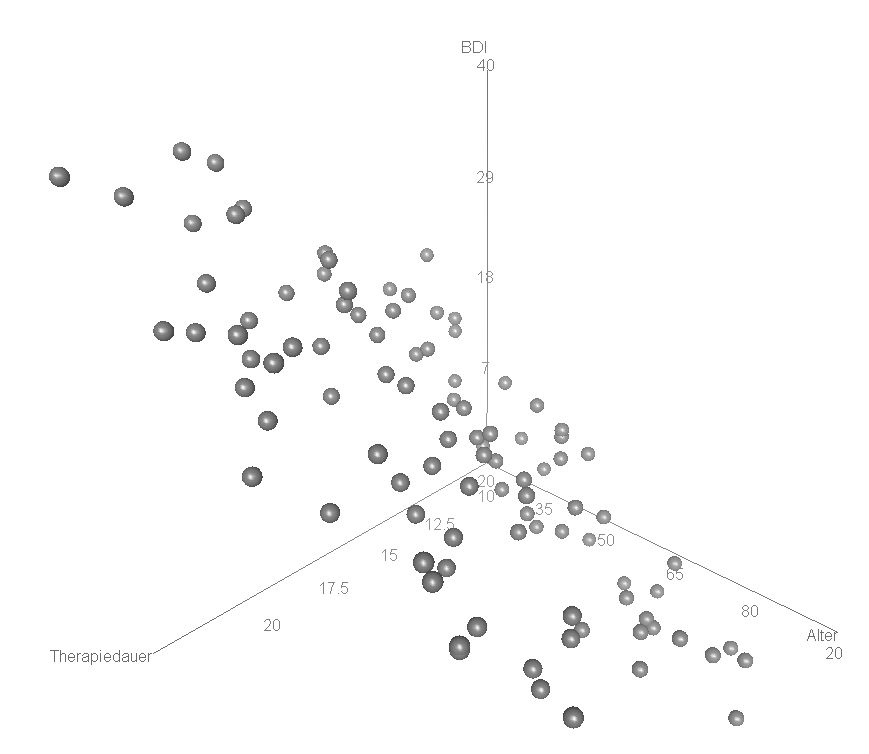
\includegraphics[width=0.6\linewidth]{12_Abbildungen/alm_2_beispieldatensatz} \end{center}
\end{frame}

\begin{frame}{}
\protect\hypertarget{section-6}{}
\large
\setstretch{2}
\vfill

Anwendungsszenario

Modellformulierung

\textbf{Modellschätzung}

Modellevaluation

Ausblick

Selbstkontrollfragen \vfill
\end{frame}

\begin{frame}{Modellschätzung}
\protect\hypertarget{modellschuxe4tzung-2}{}
\textcolor{darkblue}{Überblick}

\small

Der Betaparameterschätzer hat bekanntlich die Form \begin{equation}
\hat{\beta} := (X^TX)^{-1}X^Ty
\end{equation} Dabei quantifizieren in sehr grober Auflösung

\begin{itemize}
\tightlist
\item
  \(X^Ty \in \mathbb{R}^p\) die Kovariation der Regressoren mit den
  Daten und
\item
  \(X^TX \in \mathbb{R}^{p \times p}\) die Kovariation der Regressoren
  untereinander.
\end{itemize}

Damit ergibt sich für die Betaparameterschätzer also eine Interpretation
als ``regressorkovarianznormalisierte Regressordatenkovariation,''
\begin{equation}
\hat{\beta} \approx \mbox{Regressorkovarianz}^{-1} \cdot \mbox{Regresssordatenkovarianz}
\end{equation} Im Folgenden wollen wir diese Intuition am Beispiel einer
einfachen multiplen Regression mit einem Interzeptregressor und zwei
unabhängigen Variablen Regressoren vertiefen, wobei die betreffenden
Kovariationen einmal durch Stichprobenkorrelationen und einmal durch
partielle Stichprobenkorrelationen quantifiziert werden sollen.
\end{frame}

\begin{frame}{Modellschätzung}
\protect\hypertarget{modellschuxe4tzung-3}{}
\footnotesize
\begin{theorem}[Betaparameterschätzer und Korrelationen]
\justifying
\normalfont
Gegeben sei ein multiples Regressionsmodel der Form
\begin{equation}
y = X\beta + \varepsilon, \varepsilon \sim N(0_n,\sigma^2I_n)
\mbox{ mit }
X
:=
\begin{pmatrix}
1      & x_{11} & x_{12} \\
\vdots & \vdots & \vdots \\
1      & x_{n1} & x_{n2} \\
\end{pmatrix}
\mbox{ und }
\beta
:=
\begin{pmatrix}
\beta_0 \\
\beta_1 \\
\beta_2
\end{pmatrix}.
\end{equation}
Dann gilt
\begin{equation}
\renewcommand{\arraystretch}{1.8}
\hat{\beta}
=
\begin{pmatrix}
\bar{y} - \hat{\beta}_1\bar{x}_1 - \hat{\beta}_2\bar{x}_2                        \\
\frac{r_{y,x_1} - r_{y,x_2}r_{x_1,x_2}}{1 - r_{x_1,x_2}^2} \frac{s_{y}}{s_{x_1}} \\
\frac{r_{y,x_2} - r_{y,x_1}r_{x_1,x_2}}{1 - r_{x_1,x_2}^2} \frac{s_{y}}{s_{x_2}} \\
\end{pmatrix},
\end{equation}
wobei für die $y_i,x_{i1}$ und $x_{i2}$ mit $i = 1,...,n$ $\bar{\cdot}$, $s_{\cdot}$
und $r_{\cdot,\cdot}$ die entsprechenden Stichprobenmittel, Stichprobenstandardabweichungen,
und Stichprobenkorrelationen bezeichnen.
\end{theorem}

Bemerkung

\begin{itemize}
\tightlist
\item
  \justifying In Bezug auf die Regressoren sind die Begriffe
  Stichprobenmittel, Stichprobenstandardabweichung, und
  Stichprobenkorrelation lediglich formal gemeint, nach Voraussetzung
  des ALMs sind die Regressorenwerte keine Realisierungen von
  Zufallsvariablen.
\end{itemize}
\end{frame}

\begin{frame}{Modellschätzung}
\protect\hypertarget{modellschuxe4tzung-4}{}
\footnotesize

\underline{Beweis}

Wir erinnern zunächst daran, dass die Form des Betaparameterschätzers
bekanntlich zum System der Normalengleichungen äquivalent ist (vgl. (6)
Modellschätzung), \begin{equation}
\hat{\beta} = (X^TX)^{-1}X^Ty \Leftrightarrow X^TX\hat{\beta} = X^Ty.
\end{equation} Ausschreiben des Normalengleichungssystems für den hier
betrachteten ALM Spezialfall ergibt dann zunächst \tiny \begin{align*}
\renewcommand{\arraystretch}{1.5}
\begin{split}
X^TX\hat{\beta} & = X^Ty
\\\Leftrightarrow
\begin{pmatrix}
1      & \cdots & 1      \\
x_{11} & \cdots & x_{n1} \\
x_{12} & \cdots & x_{n2} \\
\end{pmatrix}
\begin{pmatrix}
1      & x_{11} & x_{12} \\
\vdots & \vdots & \vdots \\
1      & x_{n1} & x_{n2} \\
\end{pmatrix}
\begin{pmatrix}
\hat{\beta}_0 \\
\hat{\beta}_1 \\
\hat{\beta}_2 \\
\end{pmatrix}
& =
\begin{pmatrix}
1      & \cdots & 1      \\
x_{11} & \cdots & x_{n1} \\
x_{12} & \cdots & x_{n2} \\
\end{pmatrix}
\begin{pmatrix}
y_1    \\
\vdots \\
y_n
\end{pmatrix}
\\\Leftrightarrow
\begin{pmatrix*}[l]
n                   & \sum_{i=1}^n x_{i1}       & \sum_{i=1}^n x_{i2}       \\
\sum_{i=1}^n x_{i1} & \sum_{i=1}^n x_{i1}^2     & \sum_{i=1}^n x_{i1}x_{i2} \\
\sum_{i=1}^n x_{i2} & \sum_{i=1}^n x_{i2}x_{i1} & \sum_{i=1}^n x_{i2}^2       \\
\end{pmatrix*}
\begin{pmatrix}
\hat{\beta}_0 \\
\hat{\beta}_1 \\
\hat{\beta}_2 \\
\end{pmatrix}
& =
\begin{pmatrix*}[l]
\sum_{i=1}^n y_i \\
\sum_{i=1}^n y_ix_{i1} \\
\sum_{i=1}^n y_ix_{i2} \\
\end{pmatrix*}
\\\Leftrightarrow
\begin{pmatrix*}[l]
n                   & \sum_{i=1}^n x_{i1}       & \sum_{i=1}^n x_{i2}       \\
\sum_{i=1}^n x_{i1} & \sum_{i=1}^n x_{i1}^2     & \sum_{i=1}^n x_{i1}x_{i2} \\
\sum_{i=1}^n x_{i2} & \sum_{i=1}^n x_{i2}x_{i1} & \sum_{i=1}^n x_{i2}^2       \\
\end{pmatrix*}
\begin{pmatrix}
\hat{\beta}_0 \\
\hat{\beta}_1 \\
\hat{\beta}_2 \\
\end{pmatrix}
& =
\begin{pmatrix*}[l]
\sum_{i=1}^n y_i \\
\sum_{i=1}^n y_ix_{i1} \\
\sum_{i=1}^n y_ix_{i2} \\
\end{pmatrix*}
\end{split}
\end{align*}
\end{frame}

\begin{frame}{Modellschätzung}
\protect\hypertarget{modellschuxe4tzung-5}{}
\footnotesize

\underline{Beweis (fortgeführt)}

und damit \tiny \begin{align*}
\renewcommand{\arraystretch}{1.5}
\begin{split}
X^TX\hat{\beta}
& =
X^Ty
\\\Leftrightarrow
\begin{pmatrix*}
n\hat{\beta}_0 + \hat{\beta}_1\sum_{i=1}^n x_{i1} + \hat{\beta}_2\sum_{i=1}^n x_{i2} \\
\hat{\beta}_0 \sum_{i=1}^n x_{i1} +  \hat{\beta}_1 \sum_{i=1}^n x_{i1}^2 + \hat{\beta}_2 \sum_{i=1}^n x_{i1}x_{i2} \\
\hat{\beta}_0 \sum_{i=1}^n x_{i2} +  \hat{\beta}_1 \sum_{i=1}^n x_{i1}x_{i2} + \hat{\beta}_2 \sum_{i=1}^n x_{i2}^2
\end{pmatrix*}
& =
\begin{pmatrix*}[l]
\sum_{i=1}^n y_i \\
\sum_{i=1}^n y_ix_{i1} \\
\sum_{i=1}^n y_ix_{i2} \\
\end{pmatrix*}
\end{split}
\end{align*} \footnotesize Aus der Gleichung der ersten
Vektorkomponenten folgt dann direkt die Form von \(\hat{\beta}_0\) mit
\tiny \begin{align}
\begin{split}
\sum_{i=1}^n y_i
& = n\hat{\beta}_0 + \hat{\beta}_1\sum_{i=1}^n x_{i1}            + \hat{\beta}_2\sum_{i=1}^n x_{i2}
\\\Leftrightarrow
\frac{1}{n}\sum_{i=1}^n y_i
& = \hat{\beta}_0  + \hat{\beta}_1\frac{1}{n}\sum_{i=1}^n x_{i1} + \hat{\beta}_2\frac{1}{n}\sum_{i=1}^n x_{i2}
\\\Leftrightarrow
\hat{\beta}_0
& = \bar{y} - \hat{\beta}_1\bar{x}_1 - \hat{\beta}_2\bar{x}_2
\end{split}
\end{align}
\end{frame}

\begin{frame}{Modellschätzung}
\protect\hypertarget{modellschuxe4tzung-6}{}
\footnotesize

\underline{Beweis (fortgeführt)}

Einsetzen dieser Form von \(\hat{\beta}_0\) in die Gleichung der zweiten
Vektorkomponenten ergibt dann \tiny \begin{align*}
\begin{split}
   \hat{\beta}_0 \sum_{i=1}^n x_{i1}
+ \hat{\beta}_1 \sum_{i=1}^n x_{i1}^2
+ \hat{\beta}_2 \sum_{i=1}^n x_{i1}x_{i2}
&
= \sum_{i=1}^n y_ix_{i1}
\\
  (\bar{y} - \hat{\beta}_1\bar{x}_1 - \hat{\beta}_2\bar{x}_2) \sum_{i=1}^n x_{i1}
+ \hat{\beta}_1 \sum_{i=1}^n x_{i1}^2
+ \hat{\beta}_2 \sum_{i=1}^n x_{i1}x_{i2}
&
= \sum_{i=1}^n y_ix_{i1}
\\
  \bar{y}\sum_{i=1}^n x_{i1}
- \hat{\beta}_1\bar{x}_1\sum_{i=1}^n x_{i1}
- \hat{\beta}_2\bar{x}_2\sum_{i=1}^n x_{i1}
+ \hat{\beta}_1 \sum_{i=1}^n x_{i1}^2
+ \hat{\beta}_2 \sum_{i=1}^n x_{i1}x_{i2}
&
= \sum_{i=1}^n y_ix_{i1}
\\
  \hat{\beta}_1 \sum_{i=1}^n x_{i1}^2
- \hat{\beta}_1\bar{x}_1\sum_{i=1}^n x_{i1}
+ \hat{\beta}_2 \sum_{i=1}^n x_{i1}x_{i2}
- \hat{\beta}_2\bar{x}_2\sum_{i=1}^n x_{i1}
&
=
  \sum_{i=1}^n y_ix_{i1}
- \bar{y}\sum_{i=1}^n x_{i1}
\\
  \hat{\beta}_1 \left(\sum_{i=1}^n x_{i1}^2     - \bar{x}_1\sum_{i=1}^n x_{i1}\right)
+ \hat{\beta}_2 \left(\sum_{i=1}^n x_{i1}x_{i2} - \bar{x}_2\sum_{i=1}^n x_{i1} \right)
&
=
  \sum_{i=1}^n y_ix_{i1}
- \bar{y}\sum_{i=1}^n x_{i1}
\end{split}
\end{align*}
\end{frame}

\begin{frame}{Modellschätzung}
\protect\hypertarget{modellschuxe4tzung-7}{}
\footnotesize

\underline{Beweis (fortgeführt)}

Im Beweis des Theorems zur Ausgleichsgerade (vgl. (1) Regression) haben
wir gesehen, dass \begin{align}
\begin{split}
\sum_{i=1}^n x_{i1}x_{i1} - \bar{x}_1\sum_{i=1}^n x_{i1} & = \sum_{i=1}^n (x_{i1} - \bar{x}_1)(x_{i1} - \bar{x}_1) \\
\sum_{i=1}^n x_{i1}x_{i2} - \bar{x}_2\sum_{i=1}^n x_{i1} & = \sum_{i=1}^n (x_{i1} - \bar{x}_1)(x_{i2} - \bar{x}_2) \\
\sum_{i=1}^n y_ix_{i1}    - \bar{y}  \sum_{i=1}^n x_{i1} & = \sum_{i=1}^n (y_i    - \bar{y}  )(x_{i1} - \bar{x}_1)
\end{split}
\end{align} \footnotesize
\end{frame}

\begin{frame}{Modellschätzung}
\protect\hypertarget{modellschuxe4tzung-8}{}
\footnotesize

\underline{Beweis (fortgeführt)}

Es ergibt sich also, dass \tiny \begin{align}
\begin{split}
  \hat{\beta}_1 \sum_{i=1}^n (x_{i1}-\bar{x}_1)(x_{i1}-\bar{x}_1)
+ \hat{\beta}_2 \sum_{i=1}^n (x_{i1}-\bar{x}_1)(x_{i2}-\bar{x}_2)
&
= \sum_{i=1}^n (y_i-\bar{y})(x_{i1}-\bar{x}_1)
\\
  \hat{\beta}_1 \frac{\sum_{i=1}^n (x_{i1}-\bar{x}_1)(x_{i1}-\bar{x}_1)}{n-1}
+ \hat{\beta}_2 \frac{\sum_{i=1}^n (x_{i1}-\bar{x}_1)(x_{i2}-\bar{x}_2)}{n-1}
&
= \frac{\sum_{i=1}^n (y_i-\bar{y})(x_{i1}-\bar{x}_1)}{n-1}
\end{split}
\end{align} \footnotesize Mit den Definitionen von
Stichprobenstandardabweichung und -korrelation folgt dann weiter \tiny
\begin{align}
\begin{split}
  \hat{\beta}_1  s_{x_1}s_{x_1}
+ \hat{\beta}_2c_{x_1,x_2}
&
= c_{y,x_1}
\\
  \hat{\beta}_1  \frac{s_{x_1}s_{x_1}}{s_ys_{x_1}}
+ \hat{\beta}_2  \frac{c_{x_1,x_2}}{s_ys_{x_1}}
&
= \frac{c_{y,x_1}}{s_ys_{x_1}}
\\
  \hat{\beta}_1  \frac{s_{x_1}}{s_y}
+ \hat{\beta}_2  \frac{c_{x_1,x_2}}{s_ys_{x_1}}
&
= r_{y,x_1}
\\
  \hat{\beta}_1  \frac{s_{x_1}}{s_y}
+ \hat{\beta}_2  \frac{c_{x_1,x_2}s_{x_2}}{s_ys_{x_1}s_{x_2}}
&
= r_{y,x_1}
\\
  \hat{\beta}_1  \frac{s_{x_1}}{s_y}
+ \hat{\beta}_2  \frac{s_{x_2}}{s_y}r_{x_1,x_2}
&
= r_{y,x_1}
\end{split}
\end{align}
\end{frame}

\begin{frame}{Modellschätzung}
\protect\hypertarget{modellschuxe4tzung-9}{}
\footnotesize

\underline{Beweis (fortgeführt)}

Definition von \begin{equation}\label{eq:sbeta}
b_j  := \frac{s_{x_j}}{s_{y}}, j = 1,2
\end{equation} erlaubt dann die Schreibweise \begin{equation}
b_1 + b_2 r_{x_1,x_2} = r_{y,x_1}.
\end{equation} Schließlich folgt analog durch Vertauschen der Subskripte
aus der Gleichung der dritten Vektorkomponenten \begin{equation}
b_1r_{x_1,x_2} + b_2  = r_{y,x_2}
\end{equation} Insgesamt haben wir also gesehen, dass die Definition des
Betaparameterschätzers im vorliegenden ALM Spezialfall ergibt, dass mit
\begin{equation}\label{eq:sbeta}
\hat{\beta}_j  = b_j \frac{s_{y}}{s_{x_j}}, j = 1,2
\end{equation} gilt, dass \begin{align}
\begin{split}
r_{y,x_1} & = b_1 + b_2 r_{x_1,x_2} \\
r_{y,x_2} & = b_1r_{x_1,x_2} + b_2
\end{split}
\end{align}
\end{frame}

\begin{frame}{Modellschätzung}
\protect\hypertarget{modellschuxe4tzung-10}{}
\footnotesize

\underline{Beweis (fortgeführt)}

Damit folgt aus der zweiten Gleichung dann sofort \begin{equation}
b_2 = r_{y,x_2} - b_1r_{x_1,x_2}.
\end{equation} Einsetzen in die erste Gleichung ergibt dann
\begin{align}
\begin{split}
b_1 + (r_{y,x_2} - b_1r_{x_1,x_2}) r_{x_1,x_2} & = r_{y,x_1}
\\
\Leftrightarrow
b_1 + r_{y,x_2}r_{x_1,x_2} - b_1r_{x_1,x_2}^2  & = r_{y,x_1}
\\
\Leftrightarrow
r_{y,x_2}r_{x_1,x_2} + b_1\left(1 - r_{x_1,x_2}^2\right) & = r_{y,x_1}
\\
\Leftrightarrow
b_1\left(1 - r_{x_1,x_2}^2\right) & = r_{y,x_1} -  r_{y,x_2}r_{x_1,x_2}
\\
\Leftrightarrow
b_1 & = \frac{r_{y,x_1} -  r_{y,x_2}r_{x_1,x_2}}{1 - r_{x_1,x_2}^2}
\end{split}
\end{align}
\end{frame}

\begin{frame}{Modellschätzung}
\protect\hypertarget{modellschuxe4tzung-11}{}
\footnotesize

\underline{Beweis (fortgeführt)}

Für \(b_2\) ergibt sich damit weiterhin \begin{align}
\begin{split}
b_2 & = r_{y,x_2} - b_1r_{x_1,x_2}
\\
\Leftrightarrow
b_2 & = r_{y,x_2} - \left(\frac{r_{y,x_1} -  r_{y,x_2}r_{x_1,x_2}}{1 - r_{x_1,x_2}^2}\right)r_{x_1,x_2}
\\
\Leftrightarrow
b_2 & = \frac{r_{y,x_2}\left(1 - r_{x_1,x_2}^2\right)}{1 - r_{x_1,x_2}^2} - \frac{r_{y,x_1}r_{x_1,x_2} -  r_{y,x_2}r_{x_1,x_2}^2}{1 - r_{x_1,x_2}^2}
\\
\Leftrightarrow
b_2 & = \frac{r_{y,x_2} - r_{y,x_2}r_{x_1,x_2}^2 - r_{y,x_1}r_{x_1,x_2} +  r_{y,x_2}r_{x_1,x_2}^2}{1 - r_{x_1,x_2}^2}
\\
\Leftrightarrow
b_2 & = \frac{r_{y,x_2} - r_{y,x_1}r_{x_1,x_2}}{1 - r_{x_1,x_2}^2}
\end{split}
\end{align} Damit folgen dann aber \begin{align}
\begin{split}
\hat{\beta}_1 & = b_1 \frac{s_{y}}{s_{x_1}} = \left(\frac{r_{y,x_1} - r_{y,x_2}r_{x_1,x_2}}{1 - r_{x_1,x_2}^2} \right) \frac{s_{y}}{s_{x_1}} \\
\hat{\beta}_2 & = b_2 \frac{s_{y}}{s_{x_2}} = \left(\frac{r_{y,x_2} - r_{y,x_1}r_{x_1,x_2}}{1 - r_{x_1,x_2}^2} \right) \frac{s_{y}}{s_{x_2}} \\
\end{split}
\end{align} und es ist alles gezeigt. \(\hfill\Box\)
\end{frame}

\begin{frame}[fragile]{Modellschätzung}
\protect\hypertarget{modellschuxe4tzung-12}{}
\textcolor{darkblue}{Anwendungsbeispiel} \tiny \vspace{1mm}
\setstretch{1.2}

\begin{Shaded}
\begin{Highlighting}[]
\CommentTok{\# Dateneinlesen}
\NormalTok{fname      }\OtherTok{=} \FunctionTok{file.path}\NormalTok{(}\FunctionTok{getwd}\NormalTok{(), }\StringTok{"12\_Daten"}\NormalTok{, }\StringTok{"12\_Multiple\_Regression\_Daten.csv"}\NormalTok{)}
\NormalTok{D          }\OtherTok{=} \FunctionTok{read.table}\NormalTok{(fname, }\AttributeTok{sep =} \StringTok{","}\NormalTok{, }\AttributeTok{header =} \ConstantTok{TRUE}\NormalTok{)         }\CommentTok{\# Datensatz}

\CommentTok{\# Modellschätzung}
\NormalTok{y          }\OtherTok{=}\NormalTok{ D}\SpecialCharTok{$}\NormalTok{BDI                                               }\CommentTok{\# Abhängige Variable}
\NormalTok{n          }\OtherTok{=} \FunctionTok{length}\NormalTok{(y)                                           }\CommentTok{\# Anzahl Datenpunkte}
\NormalTok{X          }\OtherTok{=} \FunctionTok{matrix}\NormalTok{(}\FunctionTok{c}\NormalTok{(}\FunctionTok{rep}\NormalTok{(}\DecValTok{1}\NormalTok{,n), D}\SpecialCharTok{$}\NormalTok{Age, D}\SpecialCharTok{$}\NormalTok{Therapy), }\AttributeTok{nrow =}\NormalTok{ n)     }\CommentTok{\# Desigmatrix}
\NormalTok{beta\_hat   }\OtherTok{=} \FunctionTok{solve}\NormalTok{(}\FunctionTok{t}\NormalTok{(X) }\SpecialCharTok{\%*\%}\NormalTok{ X) }\SpecialCharTok{\%*\%} \FunctionTok{t}\NormalTok{(X) }\SpecialCharTok{\%*\%}\NormalTok{ y                    }\CommentTok{\# Betaparameterschätzer}
\NormalTok{eps\_hat    }\OtherTok{=}\NormalTok{ y }\SpecialCharTok{{-}}\NormalTok{ X }\SpecialCharTok{\%*\%}\NormalTok{ beta\_hat                                  }\CommentTok{\# Residuenvektor}
\NormalTok{sigsqr\_hat }\OtherTok{=}\NormalTok{ (}\FunctionTok{t}\NormalTok{(eps\_hat) }\SpecialCharTok{\%*\%}\NormalTok{ eps\_hat) }\SpecialCharTok{/}\NormalTok{(n}\SpecialCharTok{{-}}\NormalTok{p)                     }\CommentTok{\# Varianzparameterschätzer}

\CommentTok{\# Betaparameterschätzer aus Stichprobenmittel, {-}standardabweichungen und {-}korrelationen}
\NormalTok{y12        }\OtherTok{=} \FunctionTok{cbind}\NormalTok{(y,X[,}\SpecialCharTok{{-}}\DecValTok{1}\NormalTok{])                                     }\CommentTok{\# y,x\_1,x\_2 Matrix}
\NormalTok{bars       }\OtherTok{=} \FunctionTok{apply}\NormalTok{(y12, }\DecValTok{2}\NormalTok{, mean)                                 }\CommentTok{\# Stichprobenmittel}
\NormalTok{s          }\OtherTok{=} \FunctionTok{apply}\NormalTok{(y12, }\DecValTok{2}\NormalTok{, sd)                                   }\CommentTok{\# Stichprobenstandardabweichungen}
\NormalTok{r          }\OtherTok{=} \FunctionTok{cor}\NormalTok{(y12)                                            }\CommentTok{\# Stichprobenkorrelationen}
\NormalTok{beta\_hat\_1 }\OtherTok{=}\NormalTok{ (r[}\DecValTok{1}\NormalTok{,}\DecValTok{2}\NormalTok{] }\SpecialCharTok{{-}}\NormalTok{ r[}\DecValTok{1}\NormalTok{,}\DecValTok{3}\NormalTok{]}\SpecialCharTok{*}\NormalTok{r[}\DecValTok{2}\NormalTok{,}\DecValTok{3}\NormalTok{])}\SpecialCharTok{/}\NormalTok{(}\DecValTok{1} \SpecialCharTok{{-}}\NormalTok{ r[}\DecValTok{2}\NormalTok{,}\DecValTok{3}\NormalTok{]}\SpecialCharTok{\^{}}\DecValTok{2}\NormalTok{)}\SpecialCharTok{*}\NormalTok{(s[}\DecValTok{1}\NormalTok{]}\SpecialCharTok{/}\NormalTok{s[}\DecValTok{2}\NormalTok{]) }\CommentTok{\# \textbackslash{}hat\{\textbackslash{}beta\}\_1}
\NormalTok{beta\_hat\_2 }\OtherTok{=}\NormalTok{ (r[}\DecValTok{1}\NormalTok{,}\DecValTok{3}\NormalTok{] }\SpecialCharTok{{-}}\NormalTok{ r[}\DecValTok{1}\NormalTok{,}\DecValTok{2}\NormalTok{]}\SpecialCharTok{*}\NormalTok{r[}\DecValTok{2}\NormalTok{,}\DecValTok{3}\NormalTok{])}\SpecialCharTok{/}\NormalTok{(}\DecValTok{1} \SpecialCharTok{{-}}\NormalTok{ r[}\DecValTok{2}\NormalTok{,}\DecValTok{3}\NormalTok{]}\SpecialCharTok{\^{}}\DecValTok{2}\NormalTok{)}\SpecialCharTok{*}\NormalTok{(s[}\DecValTok{1}\NormalTok{]}\SpecialCharTok{/}\NormalTok{s[}\DecValTok{3}\NormalTok{]) }\CommentTok{\# \textbackslash{}hat\{\textbackslash{}beta\}\_2}
\NormalTok{beta\_hat\_0 }\OtherTok{=}\NormalTok{ bars[}\DecValTok{1}\NormalTok{] }\SpecialCharTok{{-}}\NormalTok{ beta\_hat\_1}\SpecialCharTok{*}\NormalTok{bars[}\DecValTok{2}\NormalTok{] }\SpecialCharTok{{-}}\NormalTok{ beta\_hat\_2}\SpecialCharTok{*}\NormalTok{bars[}\DecValTok{3}\NormalTok{]   }\CommentTok{\# \textbackslash{}hat\{\textbackslash{}beta\}\_0}

\CommentTok{\# Ausgabe}
\FunctionTok{cat}\NormalTok{(}\StringTok{"beta\_hat ALM{-}Schätzer          :"}\NormalTok{  , beta\_hat,}
    \StringTok{"}\SpecialCharTok{\textbackslash{}n}\StringTok{beta\_hat Deskriptivstatistiken :"}\NormalTok{, }\FunctionTok{c}\NormalTok{(beta\_hat\_0,beta\_hat\_1,beta\_hat\_2))}
\end{Highlighting}
\end{Shaded}

\begin{verbatim}
> beta_hat ALM-Schätzer          : 5.42 -0.481 1.91 
> beta_hat Deskriptivstatistiken : 5.42 -0.481 1.91
\end{verbatim}
\end{frame}

\begin{frame}[fragile]{Modellschätzung}
\protect\hypertarget{modellschuxe4tzung-13}{}
\vspace{2mm}

\textcolor{darkblue}{Beispieldatenvisualisierung} \vspace{1mm} \tiny
\setstretch{1.2}

\begin{Shaded}
\begin{Highlighting}[]
\CommentTok{\# Dateneinlesen}
\NormalTok{fname      }\OtherTok{=} \FunctionTok{file.path}\NormalTok{(}\FunctionTok{getwd}\NormalTok{(), }\StringTok{"12\_Daten"}\NormalTok{, }\StringTok{"12\_Multiple\_Regression\_Daten.csv"}\NormalTok{)}
\NormalTok{D          }\OtherTok{=} \FunctionTok{read.table}\NormalTok{(fname, }\AttributeTok{sep =} \StringTok{","}\NormalTok{, }\AttributeTok{header =} \ConstantTok{TRUE}\NormalTok{)         }\CommentTok{\# Datensatz}

\CommentTok{\# Open GL Visualisierung  mit car package, siehe ?scatter3d für Details}
\FunctionTok{library}\NormalTok{(car)}
\FunctionTok{scatter3d}\NormalTok{(}
\NormalTok{D}\SpecialCharTok{$}\NormalTok{Age,}
\NormalTok{D}\SpecialCharTok{$}\NormalTok{BDI,}
\NormalTok{D}\SpecialCharTok{$}\NormalTok{Therapy,}
\AttributeTok{xlab        =} \StringTok{"Alter"}\NormalTok{,}
\AttributeTok{ylab        =} \StringTok{"BDI"}\NormalTok{,}
\AttributeTok{zlab        =} \StringTok{"Therapiedauer"}\NormalTok{,}
\AttributeTok{point.col   =} \StringTok{"gray40"}\NormalTok{,}
\AttributeTok{axis.col    =} \FunctionTok{rep}\NormalTok{(}\StringTok{"black"}\NormalTok{,}\DecValTok{3}\NormalTok{),}
\AttributeTok{axis.scales =}\NormalTok{ T,}
\AttributeTok{axis.ticks  =}\NormalTok{ T,}
\AttributeTok{surface     =}\NormalTok{ T,}
\AttributeTok{surface.col =} \StringTok{"gray70"}\NormalTok{,}
\AttributeTok{neg.res.col =} \StringTok{"gray70"}\NormalTok{,}
\AttributeTok{pos.res.col =} \StringTok{"gray70"}\NormalTok{)}
\end{Highlighting}
\end{Shaded}
\end{frame}

\begin{frame}{Modellschätzung}
\protect\hypertarget{modellschuxe4tzung-14}{}
\vspace{2mm}

\textcolor{darkblue}{Beispieldatenvisualisierung} \vspace{1mm}

\center

\begin{center}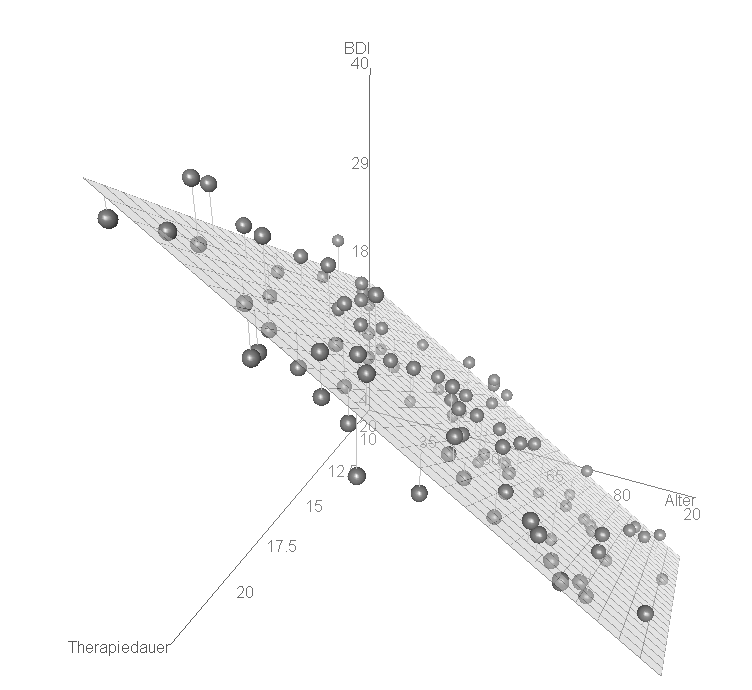
\includegraphics[width=0.6\linewidth]{12_Abbildungen/alm_2_beispieldatensatz_fit} \end{center}
\end{frame}

\begin{frame}{Modellschätzung}
\protect\hypertarget{modellschuxe4tzung-15}{}
\footnotesize
\begin{theorem}[Betaparameterschätzer und partielle Korrelationen]
\justifying
\normalfont
Gegeben sei ein multiples Regressionsmodel der Form
\begin{equation}
y = X\beta + \varepsilon, \varepsilon \sim N(0_n,\sigma^2I_n)
\mbox{ mit }
X
:=
\begin{pmatrix}
1      & x_{11} & x_{12} \\
\vdots & \vdots & \vdots \\
1      & x_{n1} & x_{n2} \\
\end{pmatrix}
\mbox{ und }
\beta
:=
\begin{pmatrix}
\beta_0 \\
\beta_1 \\
\beta_2
\end{pmatrix}.
\end{equation}
Dann gilt
\begin{equation}
\hat{\beta}
=
\begin{pmatrix}
\bar{y} - \hat{\beta}_1\bar{x}_1 - \hat{\beta}_2\bar{x}_2     \\
r_{y,x_1|x_2}\sqrt{\frac{1-r^2_{y,x_2}}{\,1-r_{x_1,x_2}^2}}\frac{s_{y}}{s_{x_1}} \\
r_{y,x_2|x_1}\sqrt{\frac{1-r^2_{y,x_1}}{\,1-r_{x_2,x_1}^2}}\frac{s_{y}}{s_{x_2}} \\
\end{pmatrix},
\end{equation}
wobei für $1 \le k,l \le 2$ und $i = 1,...,n$
\begin{itemize}
\item $r_{y,x_k|x_l}$ die partielle Stichprobenkorrelation der  $y_i$ und $x_{ik}$ gegeben die $x_{il}$ ist,
\item $r_{y,x_k}$ die Stichprobenkorrelation der $y_i$ und $x_{ik}$ ist, und
\item $r_{x_k,x_l}$ die Stichprobenkorrelation der $x_{ik}$ und $x_{il}$ ist.
\end{itemize}
\end{theorem}
\end{frame}

\begin{frame}{Modellschätzung}
\protect\hypertarget{modellschuxe4tzung-16}{}
\small

Bemerkungen

\begin{itemize}
\item Im Allgemeinen gilt für $1 \le i,l \le k$, dass $\hat{\beta}_k \neq r_{y,x_k|x_l}$.
\item Betaparameterschätzer sind also im Allgemeinen keine partiellen Stichprobenkorrelationen.
\item $\hat{\beta}_k = r_{y,x_k|x_l}$ für $1 \le i,l \le k$ gilt genau dann, wenn $s_y = s_{x_1} = s_{x_2}$ und zudem
\begin{itemize}
\justifying
\begin{small}
\item $r_{y,x_k} = r_{x_k,x_l} = 0$, wenn also die Stichprobenkorrelationen der Daten
      und der Werte des zweiten Regressors, sowie die Stichprobenkorrelation der Werte
      der beiden Regressoren gleich Null sind. Dies kann der Fall sein, wenn einer der
      Regressoren die Daten ``sehr gut erklärt'' und der andere Regressor von dem
      ersten ``sehr verschieden'' ist.
\item $|r_{y,x_l}| = |r_{x_k,x_l}|$, wenn also die obige Stichprobenkorrelationen
      dem Betrage nach gleich sind. Dies ist vermutlich selten der Fall.
\end{small}
\end{itemize}
\end{itemize}
\end{frame}

\begin{frame}{Modellschätzung}
\protect\hypertarget{modellschuxe4tzung-17}{}
\footnotesize

\underline{Beweis}

Wir betrachten \(\hat{\beta}_1\), das Resultat für \(\hat{\beta}_2\)
folgt dann durch Vertauschen der Indizes. Wir haben in vorherigem
Theorem gesehen, dass \begin{equation}
\hat{\beta}_1 = \frac{r_{y,x_1} - r_{y,x_2}r_{x_1,x_2}}{1 - r_{x_1,x_2}^2} \frac{s_{y}}{s_{x_1}}
\end{equation} Weiterhin haben wir in (2) Korrelation gesehen, dass
unter der Annahme der multivariaten Normalverteilung von \(y,x_1,x_2\)
ein Schätzer für die partielle Kkorrelation von \(y\) und \(x_1\)
gegeben \(x_2\) durch \begin{equation}
r_{y,x_1|x_2} = \frac{r_{y,x_1} - r_{y,x_2}r_{x_1,x_2}}{\sqrt{1 - r^2_{y,x_2}}\sqrt{1 - r_{x_1,x_2}^2}}
\end{equation} gegeben ist. Für \(\hat{\beta}_1\) ergibt sich somit
\tiny \begin{align}
\begin{split}
\hat{\beta}_1
& = \frac{r_{y,x_1} - r_{y,x_2}r_{x_1,x_2}}{1 - r_{x_1,x_2}^2} \frac{s_{y}}{s_{x_1}}
\\
\Leftrightarrow
\left(1 - r_{x_1,x_2}^2\right)\hat{\beta}_1
& = (r_{y,x_1} - r_{y,x_2}r_{x_1,x_2}) \frac{s_{y}}{s_{x_1}}
\\
\Leftrightarrow
\frac{1 - r_{x_1,x_2}^2}{\sqrt{1 - r^2_{y,x_2}}\sqrt{1 - r_{x_1,x_2}^2}}\hat{\beta}_1
& = \frac{r_{y,x_1} - r_{y,x_2}r_{x_1,x_2}}{\sqrt{1 - r^2_{y,x_2}}\sqrt{1-r_{x_1,x_2}^2}} \frac{s_{y}}{s_{x_1}}
\\
\Leftrightarrow
\frac{1 - r_{x_1,x_2}^2}{\sqrt{1 - r^2_{y,x_2}}\sqrt{1 - r_{x_1,x_2}^2}}\hat{\beta}_1
& = r_{y,x_1|x_2}\frac{s_{y}}{s_{x_1}}
\end{split}
\end{align}
\end{frame}

\begin{frame}{Modellschätzung}
\protect\hypertarget{modellschuxe4tzung-18}{}
\footnotesize

\underline{Beweis}

und damit weiter \begin{align}
\begin{split}
\hat{\beta}_1
& = r_{y,x_1|x_2}\frac{\sqrt{1 - r^2_{y,x_2}}\sqrt{1 - r_{x_1,x_2}^2}}{1 - r_{x_1,x_2}^2}\frac{s_{y}}{s_{x_1}}
\\
\Leftrightarrow
\hat{\beta}_1
& = r_{y,x_1|x_2}\frac{\sqrt{1 - r^2_{y,x_2}}\sqrt{1 - r_{x_1,x_2}^2}}{\left(\sqrt{1 - r_{x_1,x_2}^2}\right)^2}\frac{s_{y}}{s_{x_1}}
\\
\Leftrightarrow
\hat{\beta}_1
& = r_{y,x_1|x_2}\frac{\sqrt{1 - r^2_{y,x_2}}}{\sqrt{1 - r_{x_1,x_2}^2}}\frac{s_{y}}{s_{x_1}}
\\
\Leftrightarrow
\hat{\beta}_1
& = r_{y,x_1|x_2}\sqrt{\frac{1 - r^2_{y,x_2}}{\,1 - r_{x_1,x_2}^2}}\frac{s_{y}}{s_{x_1}}
\end{split}
\end{align}
\end{frame}

\begin{frame}[fragile]{Modellschätzung}
\protect\hypertarget{modellschuxe4tzung-19}{}
\textcolor{darkblue}{Anwendungsbeispiel} \tiny \vspace{1mm}
\setstretch{.9}

\begin{Shaded}
\begin{Highlighting}[]
\CommentTok{\# Dateneinlesen}
\NormalTok{fname      }\OtherTok{=} \FunctionTok{file.path}\NormalTok{(}\FunctionTok{getwd}\NormalTok{(), }\StringTok{"12\_Daten"}\NormalTok{, }\StringTok{"12\_Multiple\_Regression\_Daten.csv"}\NormalTok{)}
\NormalTok{D          }\OtherTok{=} \FunctionTok{read.table}\NormalTok{(fname, }\AttributeTok{sep =} \StringTok{","}\NormalTok{, }\AttributeTok{header =} \ConstantTok{TRUE}\NormalTok{)         }\CommentTok{\# Datensatz}

\CommentTok{\# Modellschätzung}
\NormalTok{y          }\OtherTok{=}\NormalTok{ D}\SpecialCharTok{$}\NormalTok{BDI                                               }\CommentTok{\# Abhängige Variable}
\NormalTok{n          }\OtherTok{=} \FunctionTok{length}\NormalTok{(y)                                           }\CommentTok{\# Anzahl Datenpunkte}
\NormalTok{X          }\OtherTok{=} \FunctionTok{matrix}\NormalTok{(}\FunctionTok{c}\NormalTok{(}\FunctionTok{rep}\NormalTok{(}\DecValTok{1}\NormalTok{,n), D}\SpecialCharTok{$}\NormalTok{Age, D}\SpecialCharTok{$}\NormalTok{Therapy), }\AttributeTok{nrow =}\NormalTok{ n)     }\CommentTok{\# Desigmatrix}
\NormalTok{p          }\OtherTok{=} \FunctionTok{ncol}\NormalTok{(X)                                             }\CommentTok{\# Anzahl Parameter}
\NormalTok{beta\_hat   }\OtherTok{=} \FunctionTok{solve}\NormalTok{(}\FunctionTok{t}\NormalTok{(X) }\SpecialCharTok{\%*\%}\NormalTok{ X) }\SpecialCharTok{\%*\%} \FunctionTok{t}\NormalTok{(X) }\SpecialCharTok{\%*\%}\NormalTok{ y                    }\CommentTok{\# Betaparameterschätzer}
\NormalTok{eps\_hat    }\OtherTok{=}\NormalTok{ y }\SpecialCharTok{{-}}\NormalTok{ X }\SpecialCharTok{\%*\%}\NormalTok{ beta\_hat                                  }\CommentTok{\# Residuenvektor}
\NormalTok{sigsqr\_hat }\OtherTok{=}\NormalTok{ (}\FunctionTok{t}\NormalTok{(eps\_hat) }\SpecialCharTok{\%*\%}\NormalTok{ eps\_hat) }\SpecialCharTok{/}\NormalTok{(n}\SpecialCharTok{{-}}\NormalTok{p)                     }\CommentTok{\# Varianzparameterschätzer}

\CommentTok{\# Betaparameterschätzer aus partiellen Korrelationen und Korrelationen}
\FunctionTok{library}\NormalTok{(ppcor)                                                   }\CommentTok{\# partielle Korrelationentoolbox}
\NormalTok{y12        }\OtherTok{=} \FunctionTok{cbind}\NormalTok{(y,X[,}\SpecialCharTok{{-}}\DecValTok{1}\NormalTok{])                                     }\CommentTok{\# y,x\_1,x\_2 Matrix}
\NormalTok{bars       }\OtherTok{=} \FunctionTok{apply}\NormalTok{(y12, }\DecValTok{2}\NormalTok{, mean)                                 }\CommentTok{\# Stichprobenmittel}
\NormalTok{s          }\OtherTok{=} \FunctionTok{apply}\NormalTok{(y12, }\DecValTok{2}\NormalTok{, sd)                                   }\CommentTok{\# Stichprobenstandardabweichungen}
\NormalTok{r          }\OtherTok{=} \FunctionTok{cor}\NormalTok{(y12)                                            }\CommentTok{\# Stichprobenkorrelationen}
\NormalTok{pr         }\OtherTok{=} \FunctionTok{pcor}\NormalTok{(y12)                                           }\CommentTok{\# partielle Stichprobenkorrelationen}
\NormalTok{pr         }\OtherTok{=}\NormalTok{ pr}\SpecialCharTok{$}\NormalTok{estimate                                         }\CommentTok{\# partielle Stichprobenkorrelationen}
\NormalTok{beta\_hat\_1 }\OtherTok{=}\NormalTok{ pr[}\DecValTok{1}\NormalTok{,}\DecValTok{2}\NormalTok{]}\SpecialCharTok{*}\FunctionTok{sqrt}\NormalTok{((}\DecValTok{1}\SpecialCharTok{{-}}\NormalTok{r[}\DecValTok{1}\NormalTok{,}\DecValTok{3}\NormalTok{]}\SpecialCharTok{\^{}}\DecValTok{2}\NormalTok{)}\SpecialCharTok{/}\NormalTok{(}\DecValTok{1}\SpecialCharTok{{-}}\NormalTok{r[}\DecValTok{2}\NormalTok{,}\DecValTok{3}\NormalTok{]}\SpecialCharTok{\^{}}\DecValTok{2}\NormalTok{))}\SpecialCharTok{*}\NormalTok{(s[}\DecValTok{1}\NormalTok{]}\SpecialCharTok{/}\NormalTok{s[}\DecValTok{2}\NormalTok{]) }\CommentTok{\# \textbackslash{}hat\{\textbackslash{}beta\}\_1}
\NormalTok{beta\_hat\_2 }\OtherTok{=}\NormalTok{ pr[}\DecValTok{1}\NormalTok{,}\DecValTok{3}\NormalTok{]}\SpecialCharTok{*}\FunctionTok{sqrt}\NormalTok{((}\DecValTok{1}\SpecialCharTok{{-}}\NormalTok{r[}\DecValTok{1}\NormalTok{,}\DecValTok{2}\NormalTok{]}\SpecialCharTok{\^{}}\DecValTok{2}\NormalTok{)}\SpecialCharTok{/}\NormalTok{(}\DecValTok{1}\SpecialCharTok{{-}}\NormalTok{r[}\DecValTok{3}\NormalTok{,}\DecValTok{2}\NormalTok{]}\SpecialCharTok{\^{}}\DecValTok{2}\NormalTok{))}\SpecialCharTok{*}\NormalTok{(s[}\DecValTok{1}\NormalTok{]}\SpecialCharTok{/}\NormalTok{s[}\DecValTok{3}\NormalTok{]) }\CommentTok{\# \textbackslash{}hat\{\textbackslash{}beta\}\_2}
\NormalTok{beta\_hat\_0 }\OtherTok{=}\NormalTok{ bars[}\DecValTok{1}\NormalTok{] }\SpecialCharTok{{-}}\NormalTok{ beta\_hat\_1}\SpecialCharTok{*}\NormalTok{bars[}\DecValTok{2}\NormalTok{] }\SpecialCharTok{{-}}\NormalTok{ beta\_hat\_2}\SpecialCharTok{*}\NormalTok{bars[}\DecValTok{3}\NormalTok{]   }\CommentTok{\# \textbackslash{}hat\{\textbackslash{}beta\}\_0}

\CommentTok{\# Ausgabe}
\FunctionTok{cat}\NormalTok{(}\StringTok{"Korrelationen  r(y,x\_1),r(y,x\_2),r(x\_1,x\_2)        :"}\NormalTok{  , }\FunctionTok{c}\NormalTok{(r[}\DecValTok{1}\NormalTok{,}\DecValTok{2}\NormalTok{],r[}\DecValTok{1}\NormalTok{,}\DecValTok{3}\NormalTok{],r[}\DecValTok{2}\NormalTok{,}\DecValTok{3}\NormalTok{]),}
    \StringTok{"}\SpecialCharTok{\textbackslash{}n}\StringTok{Partielle Korrelationen r(y,x\_1|x\_2), r(y,x\_2|x\_1) :"}\NormalTok{, }\FunctionTok{c}\NormalTok{(pr[}\DecValTok{1}\NormalTok{,}\DecValTok{2}\NormalTok{],pr[}\DecValTok{1}\NormalTok{,}\DecValTok{3}\NormalTok{]),}
    \StringTok{"}\SpecialCharTok{\textbackslash{}n}\StringTok{beta\_hat ALM Schätzer                              :"}\NormalTok{, beta\_hat,}
    \StringTok{"}\SpecialCharTok{\textbackslash{}n}\StringTok{beta\_hat aus partieller Korrelation                :"}\NormalTok{, }\FunctionTok{c}\NormalTok{(beta\_hat\_0,beta\_hat\_1,beta\_hat\_2))}
\end{Highlighting}
\end{Shaded}

\begin{verbatim}
> Korrelationen  r(y,x_1),r(y,x_2),r(x_1,x_2)        : -0.726 0.644 -0.0268 
> Partielle Korrelationen r(y,x_1|x_2), r(y,x_2|x_1) : -0.927 0.909 
> beta_hat ALM Schätzer                              : 5.42 -0.481 1.91 
> beta_hat aus partieller Korrelation                : 5.42 -0.481 1.91
\end{verbatim}
\end{frame}

\begin{frame}{}
\protect\hypertarget{section-7}{}
\large
\setstretch{2}
\vfill

Anwendungsszenario

Modellformulierung

Modellschätzung

\textbf{Modellevaluation}

Ausblick

Selbstkontrollfragen \vfill
\end{frame}

\begin{frame}{Modellevaluation}
\protect\hypertarget{modellevaluation}{}
\textcolor{darkblue}{Parameterinferenz | T-Tests}

\small

Zur Erinnerung (vgl. (7) Modellevaluation)

\vspace{1mm}
\footnotesize
\begin{theorem}[T-Teststatistik]
\normalfont
\justifying
Es sei
\begin{equation}
y = X\beta + \varepsilon \mbox{ mit } \varepsilon \sim N(0_n,\sigma^2I_n)
\end{equation}
das ALM in generativer Form. Weiterhin seien
\begin{equation}
\hat{\beta} := (X^TX)^{-1}X^Ty \mbox{ und } \hat{\sigma}^2 := \frac{(y - X\hat{\beta})^T(y - X\hat{\beta})}{n-p}
\end{equation}
die Betaparameter- und Varianzparameterschätzer, respektive. Schließlich sei für
einen \textit{Kontrastgewichtsvektor} $c \in \mathbb{R}^p$ und
einen \textit{Nullhypothesenbetaparameter} $\beta_0 \in \mathbb{R}^p$
die \textit{T-Teststatistik} definiert als
\begin{equation}
T := \frac{c^T\hat{\beta} - c^T\beta_0}{\sqrt{\hat{\sigma}^2 c^T(X^TX)^{-1}c}}.
\end{equation}
Dann gilt
\begin{equation}
T \sim t(\delta, n-p) \mbox{ mit } \delta := \frac{c^T\beta - c^T\beta_0}{\sqrt{\sigma^2 c^T(X^TX)^{-1}c}}
\end{equation}
\end{theorem}
\end{frame}

\begin{frame}{Modellevaluation}
\protect\hypertarget{modellevaluation-1}{}
\textcolor{darkblue}{Parameterinferenz | T-Tests}

\small

Einige mögliche Kontrastgewichtsvektoren und Nullhypothesen im
Anwendungsbeispiel:

\vspace{2mm}
\center
\renewcommand{\arraystretch}{3}
\begin{tabular}{lll}
$c = (1,0,0)^T$  & $H_0 : \beta_1 = 0$           & $H_A:\beta_1 \neq 0$          \\
$c = (0,1,0)^T$  & $H_0 : \beta_2 = 0$           & $H_A:\beta_2 \neq 0$          \\
$c = (0,0,1)^T$  & $H_0 : \beta_3 = 0$           & $H_A:\beta_3 \neq 0$          \\
$c = (0,1,-1)^T$ & $H_0 : \beta_2 - \beta_3 = 0$ & $H_A:\beta_2-\beta_3\neq 0$   \\
$\cdots$         & $\cdots$                      & $\cdots$                      \\
\end{tabular}
\end{frame}

\begin{frame}[fragile]{Modellevaluation}
\protect\hypertarget{modellevaluation-2}{}
\textcolor{darkblue}{Parameterinferenz | T-Tests}

\vspace{1mm}
\tiny
\setstretch{0.9}

\begin{Shaded}
\begin{Highlighting}[]
\CommentTok{\# Dateneinlesen}
\NormalTok{fname      }\OtherTok{=} \FunctionTok{file.path}\NormalTok{(}\FunctionTok{getwd}\NormalTok{(), }\StringTok{"12\_Daten"}\NormalTok{, }\StringTok{"12\_Multiple\_Regression\_Daten.csv"}\NormalTok{)}
\NormalTok{D          }\OtherTok{=} \FunctionTok{read.table}\NormalTok{(fname, }\AttributeTok{sep =} \StringTok{","}\NormalTok{, }\AttributeTok{header =} \ConstantTok{TRUE}\NormalTok{)         }\CommentTok{\# Datensatz}

\CommentTok{\# Modellschätzung}
\NormalTok{y          }\OtherTok{=}\NormalTok{ D}\SpecialCharTok{$}\NormalTok{BDI                                            }\CommentTok{\# Abhängige Variable}
\NormalTok{n          }\OtherTok{=} \FunctionTok{length}\NormalTok{(y)                                        }\CommentTok{\# Anzahl Datenpunkte}
\NormalTok{X          }\OtherTok{=} \FunctionTok{matrix}\NormalTok{(}\FunctionTok{c}\NormalTok{(}\FunctionTok{rep}\NormalTok{(}\DecValTok{1}\NormalTok{,n), D}\SpecialCharTok{$}\NormalTok{Age, D}\SpecialCharTok{$}\NormalTok{Therapy), }\AttributeTok{nrow =}\NormalTok{ n)  }\CommentTok{\# Desigmatrix}
\NormalTok{p          }\OtherTok{=} \FunctionTok{ncol}\NormalTok{(X)                                          }\CommentTok{\# Anzahl Parameter}
\NormalTok{beta\_hat   }\OtherTok{=} \FunctionTok{solve}\NormalTok{(}\FunctionTok{t}\NormalTok{(X) }\SpecialCharTok{\%*\%}\NormalTok{ X) }\SpecialCharTok{\%*\%} \FunctionTok{t}\NormalTok{(X) }\SpecialCharTok{\%*\%}\NormalTok{ y                 }\CommentTok{\# Betaparameterschätzer}
\NormalTok{eps\_hat    }\OtherTok{=}\NormalTok{ y }\SpecialCharTok{{-}}\NormalTok{ X }\SpecialCharTok{\%*\%}\NormalTok{ beta\_hat                               }\CommentTok{\# Residuenvektor}
\NormalTok{sigsqr\_hat }\OtherTok{=}\NormalTok{ (}\FunctionTok{t}\NormalTok{(eps\_hat) }\SpecialCharTok{\%*\%}\NormalTok{ eps\_hat) }\SpecialCharTok{/}\NormalTok{(n}\SpecialCharTok{{-}}\NormalTok{p)                  }\CommentTok{\# Varianzparameterschätzer}

\CommentTok{\# Modellevaluation | Parameterinferenz}
\NormalTok{C          }\OtherTok{=} \FunctionTok{cbind}\NormalTok{(}\FunctionTok{diag}\NormalTok{(p), }\FunctionTok{matrix}\NormalTok{(}\FunctionTok{c}\NormalTok{(}\DecValTok{0}\NormalTok{,}\DecValTok{1}\NormalTok{,}\SpecialCharTok{{-}}\DecValTok{1}\NormalTok{), }\AttributeTok{nrow =} \DecValTok{3}\NormalTok{))      }\CommentTok{\# Kontrastgewichtsvektoren}
\NormalTok{ste        }\OtherTok{=} \FunctionTok{rep}\NormalTok{(}\ConstantTok{NaN}\NormalTok{, }\FunctionTok{ncol}\NormalTok{(C))                                }\CommentTok{\# Konstraststandardfehler}
\NormalTok{tee        }\OtherTok{=} \FunctionTok{rep}\NormalTok{(}\ConstantTok{NaN}\NormalTok{, }\FunctionTok{ncol}\NormalTok{(C))                                }\CommentTok{\# T{-}Statistiken}
\NormalTok{pvals      }\OtherTok{=} \FunctionTok{rep}\NormalTok{(}\ConstantTok{NaN}\NormalTok{, }\FunctionTok{ncol}\NormalTok{(C))                                }\CommentTok{\# p{-}Werte}
\ControlFlowTok{for}\NormalTok{(i }\ControlFlowTok{in} \DecValTok{1}\SpecialCharTok{:}\FunctionTok{ncol}\NormalTok{(C))\{}
\NormalTok{    c        }\OtherTok{=}\NormalTok{ C[,i]                                          }\CommentTok{\# Kontrastgewichtsvektor}
\NormalTok{    t\_num    }\OtherTok{=} \FunctionTok{t}\NormalTok{(c)}\SpecialCharTok{\%*\%}\NormalTok{beta\_hat                                }\CommentTok{\# Zähler der T{-}Statistik}
\NormalTok{    ste[i]   }\OtherTok{=} \FunctionTok{sqrt}\NormalTok{(sigsqr\_hat}\SpecialCharTok{*}\FunctionTok{t}\NormalTok{(c)}\SpecialCharTok{\%*\%}\FunctionTok{solve}\NormalTok{(}\FunctionTok{t}\NormalTok{(X)}\SpecialCharTok{\%*\%}\NormalTok{X)}\SpecialCharTok{\%*\%}\NormalTok{c)    }\CommentTok{\# Kontraststandardfehler/Nenner der T{-}Statistik}
\NormalTok{    tee[i]   }\OtherTok{=}\NormalTok{ t\_num}\SpecialCharTok{/}\NormalTok{ste[i]                                   }\CommentTok{\# T{-}Statistik}
\NormalTok{    pvals[i] }\OtherTok{=} \DecValTok{2}\SpecialCharTok{*}\NormalTok{(}\DecValTok{1} \SpecialCharTok{{-}} \FunctionTok{pt}\NormalTok{(}\FunctionTok{abs}\NormalTok{(tee[i]),n}\SpecialCharTok{{-}}\NormalTok{p))                    }\CommentTok{\# p{-}Wert}
\NormalTok{\}}
\CommentTok{\# Ausgabe}
\NormalTok{R            }\OtherTok{=} \FunctionTok{data.frame}\NormalTok{(}\FunctionTok{c}\NormalTok{(beta\_hat, }\FunctionTok{t}\NormalTok{(C[,}\DecValTok{4}\NormalTok{]}\SpecialCharTok{\%*\%}\NormalTok{beta\_hat)),ste, tee, pvals)}
\FunctionTok{rownames}\NormalTok{(R)  }\OtherTok{=} \FunctionTok{c}\NormalTok{(}\StringTok{"(Intercept)"}\NormalTok{, }\StringTok{"Age"}\NormalTok{, }\StringTok{"Therapy"}\NormalTok{, }\StringTok{"Age{-}Therapy"}\NormalTok{)}
\FunctionTok{colnames}\NormalTok{(R)  }\OtherTok{=} \FunctionTok{c}\NormalTok{(}\StringTok{"Estimate"}\NormalTok{, }\StringTok{"Std. Error"}\NormalTok{, }\StringTok{"t value"}\NormalTok{, }\StringTok{"Pr(\textgreater{}|t|)"}\NormalTok{)}
\FunctionTok{print}\NormalTok{(R)}
\end{Highlighting}
\end{Shaded}

\begin{verbatim}
>             Estimate Std. Error t value Pr(>|t|)
> (Intercept)    5.422     1.9024    2.85  0.00534
> Age           -0.481     0.0198  -24.33  0.00000
> Therapy        1.912     0.0893   21.41  0.00000
> Age-Therapy   -2.393     0.0909  -26.32  0.00000
\end{verbatim}
\end{frame}

\begin{frame}{Modellevaluation}
\protect\hypertarget{modellevaluation-3}{}
\textcolor{darkblue}{Modellinferenz | F-Tests}

\small

Zur Erinnerung (vgl. (7) Modellevaluation)

\footnotesize
\begin{theorem}[F-Statistik]
\justifying
\normalfont
Für $X \in \mathbb{R}^{n \times p}, \beta \in \mathbb{R}^p$ und $\sigma^2 > 0$
sei ein ALM der Form
\begin{equation}
y = X\beta + \varepsilon \mbox{ mit } \varepsilon \sim N(0_n,\sigma^2I_n)
\end{equation}
mit der Partitionierung
\begin{equation}
X      = \begin{pmatrix} X_1     & X_2      \end{pmatrix},
X_1      \in \mathbb{R}^{n\times p_1},
X_2      \in \mathbb{R}^{n\times p_2},
\mbox{ und }
\beta := \begin{pmatrix} \beta_1 \\ \beta_2 \end{pmatrix},
\beta_1 \in \mathbb{R}^{p_1},
\beta_2 \in \mathbb{R}^{p_2},
\end{equation}
mit $p = p_1 + p_2$ gegeben. Schließlich sei
\begin{equation}
K := \begin{pmatrix} 0_{p_1} \\ 1_{p_2} \end{pmatrix} \in \mathbb{R}^p
\end{equation}
ein Kontrastgewichtsvektor. Dann gilt
\begin{equation}
F \sim f(\delta, p_2, n-p) \mbox{ mit } \delta := \frac{K^T\beta \left(K^T(X^TX)^{-1}K\right)^{-1}K^T \beta}{\sigma^2}
\end{equation}
\end{theorem}
\end{frame}

\begin{frame}[fragile]{Modellevaluation}
\protect\hypertarget{modellevaluation-4}{}
\textcolor{darkblue}{Modellinferenz | F-Tests}

\small

\(p_1 := 1\)

\tiny
\setstretch{1.2}
\vspace{1mm}

\begin{Shaded}
\begin{Highlighting}[]
\CommentTok{\# Dateneinlesen}
\NormalTok{fname      }\OtherTok{=} \FunctionTok{file.path}\NormalTok{(}\FunctionTok{getwd}\NormalTok{(), }\StringTok{"12\_Daten"}\NormalTok{, }\StringTok{"12\_Multiple\_Regression\_Daten.csv"}\NormalTok{)}
\NormalTok{D          }\OtherTok{=} \FunctionTok{read.table}\NormalTok{(fname, }\AttributeTok{sep =} \StringTok{","}\NormalTok{, }\AttributeTok{header =} \ConstantTok{TRUE}\NormalTok{)      }\CommentTok{\# Datensatz}

\CommentTok{\# Modellevaluation}
\NormalTok{y          }\OtherTok{=}\NormalTok{ D}\SpecialCharTok{$}\NormalTok{BDI                                            }\CommentTok{\# Abhängige Variable}
\NormalTok{n          }\OtherTok{=} \FunctionTok{length}\NormalTok{(y)                                        }\CommentTok{\# Anzahl Datenpunkte}
\NormalTok{X          }\OtherTok{=} \FunctionTok{matrix}\NormalTok{(}\FunctionTok{c}\NormalTok{(}\FunctionTok{rep}\NormalTok{(}\DecValTok{1}\NormalTok{,n), D}\SpecialCharTok{$}\NormalTok{Age, D}\SpecialCharTok{$}\NormalTok{Therapy), }\AttributeTok{nrow =}\NormalTok{ n)  }\CommentTok{\# Desigmatrix vollständiges Modell}
\NormalTok{p          }\OtherTok{=} \FunctionTok{ncol}\NormalTok{(X)                                          }\CommentTok{\# Anzahl Parameter vollständiges Modell}
\NormalTok{p\_1        }\OtherTok{=} \DecValTok{1}                                                \CommentTok{\# Anzahl Parameter reduziertes Modell}
\NormalTok{p\_2        }\OtherTok{=}\NormalTok{ p }\SpecialCharTok{{-}}\NormalTok{ p\_1                                          }\CommentTok{\# Anzahl zusätzlicher Parameter im vollst. Modell}
\NormalTok{X\_1        }\OtherTok{=}\NormalTok{ X[,}\DecValTok{1}\SpecialCharTok{:}\NormalTok{p\_1]                                        }\CommentTok{\# Designmatrix reduzierters Modell}
\NormalTok{beta\_hat\_1 }\OtherTok{=} \FunctionTok{solve}\NormalTok{(}\FunctionTok{t}\NormalTok{(X\_1)}\SpecialCharTok{\%*\%}\NormalTok{X\_1)}\SpecialCharTok{\%*\%}\FunctionTok{t}\NormalTok{(X\_1)}\SpecialCharTok{\%*\%}\NormalTok{y                 }\CommentTok{\# Betaparameterschätzer reduziertes Modell}
\NormalTok{beta\_hat   }\OtherTok{=} \FunctionTok{solve}\NormalTok{(}\FunctionTok{t}\NormalTok{(X) }\SpecialCharTok{\%*\%}\NormalTok{X )}\SpecialCharTok{\%*\%}\FunctionTok{t}\NormalTok{(X) }\SpecialCharTok{\%*\%}\NormalTok{y                    }\CommentTok{\# Betaparameterschätzer vollständiges Modell}
\NormalTok{eps\_hat\_1  }\OtherTok{=}\NormalTok{ y}\SpecialCharTok{{-}}\NormalTok{X\_1}\SpecialCharTok{\%*\%}\NormalTok{beta\_hat\_1                               }\CommentTok{\# Residuenvektor reduziertes Modell}
\NormalTok{eps\_hat    }\OtherTok{=}\NormalTok{ y }\SpecialCharTok{{-}}\NormalTok{ X}\SpecialCharTok{\%*\%}\NormalTok{beta\_hat                                 }\CommentTok{\# Residuenvektor vollständiges Modell}
\NormalTok{eh1\_eh1    }\OtherTok{=} \FunctionTok{t}\NormalTok{(eps\_hat\_1) }\SpecialCharTok{\%*\%}\NormalTok{ eps\_hat\_1                       }\CommentTok{\# RQS reduziertes Modell}
\NormalTok{eh\_eh      }\OtherTok{=} \FunctionTok{t}\NormalTok{(eps\_hat) }\SpecialCharTok{\%*\%}\NormalTok{ eps\_hat                           }\CommentTok{\# RQS vollständiges Modell}
\NormalTok{sigsqr\_hat }\OtherTok{=}\NormalTok{ eh\_eh}\SpecialCharTok{/}\NormalTok{(n}\SpecialCharTok{{-}}\NormalTok{p)                                      }\CommentTok{\# Varianzparameterschätzer vollst. Modell}
\NormalTok{f          }\OtherTok{=}\NormalTok{ ((eh1\_eh1}\SpecialCharTok{{-}}\NormalTok{eh\_eh)}\SpecialCharTok{/}\NormalTok{p\_2)}\SpecialCharTok{/}\NormalTok{sigsqr\_hat                 }\CommentTok{\# F{-}Statistik}
\NormalTok{pval       }\OtherTok{=} \DecValTok{1} \SpecialCharTok{{-}} \FunctionTok{pf}\NormalTok{(f,p\_2,n}\SpecialCharTok{{-}}\NormalTok{p)                                }\CommentTok{\# p{-}Wert}

\CommentTok{\# Ausgabe}
\FunctionTok{cat}\NormalTok{(}\StringTok{"F{-}statistic:"}\NormalTok{, f, }\StringTok{"on"}\NormalTok{, p\_2, }\StringTok{"and"}\NormalTok{, n}\SpecialCharTok{{-}}\NormalTok{p, }\StringTok{"DF"}\NormalTok{, }\StringTok{"p{-}value: "}\NormalTok{, }\FunctionTok{paste}\NormalTok{(pval))}
\end{Highlighting}
\end{Shaded}

\begin{verbatim}
> F-statistic: 540 on 2 and 97 DF p-value:  0
\end{verbatim}
\end{frame}

\begin{frame}[fragile]{Modellevaluation}
\protect\hypertarget{modellevaluation-5}{}
\textcolor{darkblue}{Modellformulierung, Modellschätzung und Modellevaluation mit R}
\vspace{2mm}

\tiny
\setstretch{1.2}

\begin{Shaded}
\begin{Highlighting}[]
\NormalTok{fname  }\OtherTok{=} \FunctionTok{file.path}\NormalTok{(}\FunctionTok{getwd}\NormalTok{(), }\StringTok{"12\_Daten"}\NormalTok{, }\StringTok{"12\_Multiple\_Regression\_Daten.csv"}\NormalTok{) }\CommentTok{\# Datensatzdatei}
\NormalTok{D      }\OtherTok{=} \FunctionTok{read.table}\NormalTok{(fname, }\AttributeTok{sep =} \StringTok{","}\NormalTok{, }\AttributeTok{header =} \ConstantTok{TRUE}\NormalTok{)                        }\CommentTok{\# Datensatzeinlesen}
\NormalTok{alm    }\OtherTok{=} \FunctionTok{lm}\NormalTok{(BDI }\SpecialCharTok{\textasciitilde{}}\NormalTok{ Age }\SpecialCharTok{+}\NormalTok{ Therapy, }\AttributeTok{data =}\NormalTok{ D)                                  }\CommentTok{\# Modellformulierung und Modellschätzung}
\FunctionTok{summary}\NormalTok{(alm)}
\end{Highlighting}
\end{Shaded}

\begin{verbatim}
> 
> Call:
> lm(formula = BDI ~ Age + Therapy, data = D)
> 
> Residuals:
>    Min     1Q Median     3Q    Max 
> -7.178 -2.165  0.438  2.585  7.119 
> 
> Coefficients:
>             Estimate Std. Error t value Pr(>|t|)    
> (Intercept)   5.4225     1.9024    2.85   0.0053 ** 
> Age          -0.4815     0.0198  -24.33   <2e-16 ***
> Therapy       1.9119     0.0893   21.41   <2e-16 ***
> ---
> Signif. codes:  0 '***' 0.001 '**' 0.01 '*' 0.05 '.' 0.1 ' ' 1
> 
> Residual standard error: 3.07 on 97 degrees of freedom
> Multiple R-squared:  0.918,   Adjusted R-squared:  0.916 
> F-statistic:  540 on 2 and 97 DF,  p-value: <2e-16
\end{verbatim}
\end{frame}

\begin{frame}{}
\protect\hypertarget{section-8}{}
\large
\setstretch{2}
\vfill

Anwendungsszenario

Modellformulierung

Modellschätzung

Modellevaluation

\textbf{Ausblick}

Selbstkontrollfragen \vfill
\end{frame}

\begin{frame}{Ausblick}
\protect\hypertarget{ausblick}{}
\setstretch{1.2}

\small

Allgemeines Lineares Modell SoSe 2023

\footnotesize

\begin{itemize}
\tightlist
\item
  Konfidenzintervalle
\item
  Allgemeine Kontrasttheorie
\item
  Kovarianzanalyse
\end{itemize}

\small

Weiterführende Theorie des Allgemeinen Linearen Modells

\footnotesize

Relaxation der Unabhängigkeitsannahme der Fehlerterme

\textcolor{darkblue}{$\quad\Rightarrow$ Generalized Least Squares, Repeated-Measures Designs, ...}

Modellierung von Beta- und Varianzparametern als Zufallsvariablen

\textcolor{darkblue}{$\quad\Rightarrow$ Hierarchische lineare Modelle, linear mixed models, Bayesian estimation, Varianzkomponentenschätzung, ...}

Nichtlineare Transformationen von Erwartungswertparametern

\textcolor{darkblue}{$\quad\Rightarrow$ Generalisierte lineare Modelle, logistische Regression, neuronale Netze, ...}

Multivariate Erweiterung der Datenvariable

\textcolor{darkblue}{$\quad\Rightarrow$ Multivariate ALMs, Faktoranalyse, Strukturgleichungsmodelle, ...}

Zeitliche Erweiterung der Datenvariable

\textcolor{darkblue}{$\quad\Rightarrow$ Linear Gaussian State Space Models, Kalman Filter, Bayesian Filtering, ...}
\end{frame}

\begin{frame}{}
\protect\hypertarget{section-9}{}
\large
\setstretch{2}
\vfill

Anwendungsszenario

Modellformulierung

Modellschätzung

Modellevaluation

Ausblick

\textbf{Selbstkontrollfragen} \vfill
\end{frame}

\begin{frame}{Selbstkontrollfragen}
\protect\hypertarget{selbstkontrollfragen}{}
\footnotesize
\begin{enumerate}
\justifying
\item Erläutern Sie das Anwendungsszenario und die Ziele der multiplen Regression.
\item Definieren Sie das Modell der multiplen Regression.
\item Erläutern Sie die Begriffe Regressor, Prädiktor, Kovariate und Feature im Rahmen der multiplen Regression.
\item Erläutern Sie, warum $\hat{\beta} \approx \mbox{Regressorkovarianz}^{-1} \mbox{Regressordatenkovarianz}$ gilt.
\item Erläutern Sie den Zusammenhang zwischen Betaparameterschätzern und partieller Korrelation in einem multiplen
Regressionmodell mit Interzeptprädiktor und zwei kontinuierlichen Prädiktoren anhand der Formel
\begin{equation}
\hat{\beta}_1 = r_{y,x_1|x_2}\sqrt{\frac{1 -r_y^2,x_2}{1 -r_{x_1,x_2}^2}}\frac{s_y}{s_{x_1}}.
\end{equation}
\item $X \in \mathbb{R}^{n \times 2}$ sei die Designmatrix eines multiplen Regressionsmodells mit zwei Prädiktoren
und Betaparametervektor $\beta := (\beta_1,\beta_2)^2$. Geben Sie den Kontrastgewichtsvektor an, 
um die Nullhypothese $H_0 : \beta_1 = \beta_2$ mithilfe der T-Statistik zu testen.
\item Simulieren Sie einen Datensatz eines multiplen Regressionsmodells mit Interzept und
zwei kontinuierlichen Regressoren $x_{1},x_{2} \in \mathbb{R}^n$, wobei $x_{i2} := ax_{i1} + \xi_i$ mit $\xi_i \sim N(0,\sigma^2_{\xi})$  für  $i = 1,...,n$
sein soll. Wählen Sie für die Simulation des Datensatzes $y \in \mathbb{R}^n$ 
den wahren, aber unbekannten, Betaparametervektor $\beta = (0,1,0)^T$ und testen Sie
die Nullhypothesen $H_0 : \beta_j = 0$ für $j = 0,1,2$. Erläutern Sie Ihre Ergebnisse.
Wiederholen Sie Analyse für den wahren, aber unbekannten, Betaparametervektor $\beta = (0,0,1)^T$.
\end{enumerate}
\end{frame}

\end{document}
